% =============================================================
%  Chapter 14: Vehicle Routing Applications in Disaster Relief
%  Vehicle Routing: Problems, Methods, and Applications (2nd ed., 2014)
%  Golden, Kovacs, Wasil
%  Self-contained Beamer slides
% =============================================================
\documentclass[aspectratio=169,10pt]{beamer}

\usetheme{Madrid}
\usecolortheme{seahorse}

\usepackage[utf8]{inputenc}
\usepackage[T1]{fontenc}
\usepackage{amsmath,amssymb,amsfonts}
\usepackage{graphicx}
\usepackage{booktabs}
\usepackage{colortbl}
\usepackage{xcolor}
\usepackage{multicol}
\usepackage{listings}
\usepackage{tikz}
\usetikzlibrary{arrows.meta,positioning,shapes.geometric,fit,backgrounds}
\usepackage{pgfplots}
\pgfplotsset{compat=1.18}
\usepackage{array}
\usepackage{longtable}
\usepackage{hyperref}
\usepackage{microtype}

\graphicspath{{figures/}}

% ── listings style ──────────────────────────────────────────
\lstset{
  language=Python,
  basicstyle=\ttfamily\scriptsize,
  numbers=left,
  numberstyle=\tiny\color{gray},
  frame=single,
  backgroundcolor=\color{gray!7},
  keywordstyle=\color{blue!70!black}\bfseries,
  commentstyle=\color{green!50!black}\itshape,
  stringstyle=\color{orange!80!black},
  breaklines=true,
  showstringspaces=false,
  tabsize=4,
}

% ── colours ─────────────────────────────────────────────────
\definecolor{myblue}{RGB}{21,101,192}
\definecolor{myred}{RGB}{198,40,40}
\definecolor{mygreen}{RGB}{46,125,50}
\definecolor{mygold}{RGB}{230,126,34}
\definecolor{mypurple}{RGB}{106,27,154}

\setbeamertemplate{footline}[frame number]
\setbeamertemplate{navigation symbols}{}

% ── metadata ────────────────────────────────────────────────
\title[Ch.14: Disaster Relief VRP]
      {Chapter 14: Vehicle Routing Applications\\in Disaster Relief}
\subtitle{Vehicle Routing: Problems, Methods, and Applications\\
          2nd Edition, 2014}
\author{B.L.\ Golden \and A.\ Kovacs \and E.A.\ Wasil}
\institute{Lecture Notes --- Self-Contained Reader Edition}
\date{2014}

% =============================================================
\begin{document}
% =============================================================

% ── Title frame ─────────────────────────────────────────────
\begin{frame}
  \titlepage
\end{frame}

% ── Table of contents ───────────────────────────────────────
\begin{frame}[allowframebreaks]{Chapter Outline}
  This chapter examines how Vehicle Routing Problem (VRP) methodology can
  be adapted and applied to the unique and demanding context of
  \textbf{humanitarian logistics} and \textbf{disaster relief operations}.
  Unlike commercial routing, disaster scenarios impose extreme uncertainty,
  life-or-death priorities, and heavily constrained resources --- making
  them among the most challenging VRP variants studied in the literature.

  \medskip
  \textbf{Chapter Sections:}
  \begin{enumerate}
    \item Introduction: What makes disaster relief routing special?
    \item Phases in Disaster Management --- preparedness, response, recovery
    \item Performance Metrics in Disaster Operations --- response time, coverage, equity
    \item Commercial VRPs vs.\ Disaster Relief VRPs --- key structural differences
    \item VRP Models for Disaster Relief --- distribution and evacuation models
    \item Conclusions and Future Research Directions
  \end{enumerate}

  \medskip
  \begin{alertblock}{Why this chapter matters}
    Every year, natural and man-made disasters displace millions of people.
    The speed and fairness with which relief supplies reach affected
    populations directly determines survival rates.
    Optimisation-based routing provides a rigorous framework for making
    these life-critical decisions under severe constraints.
  \end{alertblock}
\end{frame}

% =============================================================
\section{Introduction}
% =============================================================

\begin{frame}[allowframebreaks]{Introduction: Disaster Relief and the VRP}
  The \textbf{Vehicle Routing Problem (VRP)} is the class of problems in
  which a fleet of vehicles must deliver goods from one or more depots to
  a set of geographically dispersed customers.
  In the commercial world, the guiding principle is economic efficiency:
  minimise total travel distance or operating cost.

  \medskip
  \textbf{Disaster relief operations} are an entirely different setting.
  When an earthquake, hurricane, flood, or conflict event strikes a
  population, aid agencies must:
  \begin{itemize}
    \item Deliver food, water, medicine, and shelter materials to survivors,
    \item Evacuate the injured and vulnerable from danger zones,
    \item Operate under extreme \emph{uncertainty} about demand, road
          conditions, and vehicle availability,
    \item Prioritise speed and equity of delivery over cost.
  \end{itemize}

  \medskip
  The authors --- Golden, Kovacs, and Wasil --- argue that
  \textbf{operations research, and the VRP in particular, has an important
  contribution to make} in this humanitarian domain, but that existing
  commercial models must be substantially modified before they are
  applicable.

  \framebreak

  \begin{block}{Defining the Core Problem}
    At its heart, a disaster relief VRP asks:
    \emph{Given a set of demand locations (affected communities),
    a set of supply locations (warehouses or staging areas),
    and a limited fleet of vehicles, determine routes for the vehicles
    such that relief items reach beneficiaries as quickly and fairly
    as possible.}
  \end{block}

  \medskip
  Several characteristics make disaster logistics qualitatively different
  from commercial logistics:
  \begin{enumerate}
    \item \textbf{Unknown demand:} The quantity and type of supplies
          needed at each location is not known until well after a disaster
          strikes.
    \item \textbf{Disrupted infrastructure:} Roads may be blocked,
          bridges collapsed, and communication networks down.
    \item \textbf{Urgency:} Every hour of delay can cost lives.
    \item \textbf{Heterogeneous fleet:} Trucks, helicopters, boats,
          and mules may all need to be coordinated.
    \item \textbf{Multiple, competing objectives:} Minimising time,
          maximising coverage, ensuring equitable distribution, and
          minimising cost can all pull in different directions.
  \end{enumerate}

  \framebreak

  \begin{figure}[h]
    \centering
    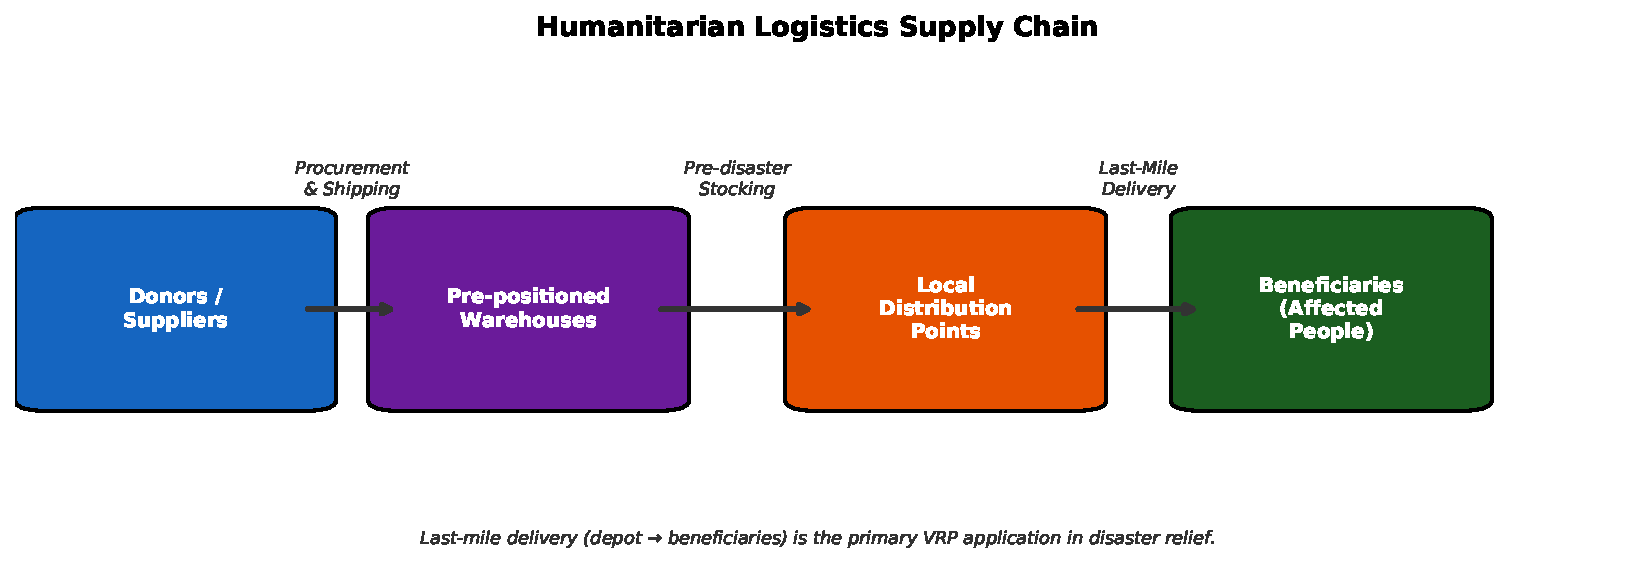
\includegraphics[width=0.72\linewidth]{fig_supply_chain.pdf}
    \caption{The humanitarian logistics supply chain from donors to
             beneficiaries. The last-mile delivery step (from local
             distribution points to affected communities) is the
             primary domain of VRP models.}
  \end{figure}

  \begin{alertblock}{Key Insight}
    The \emph{last-mile delivery} challenge --- getting supplies from a
    central point to scattered, hard-to-reach beneficiaries --- is
    precisely the problem that VRP was designed to solve.
    This is why the VRP literature has become a cornerstone of
    humanitarian logistics research.
  \end{alertblock}
\end{frame}

\begin{frame}[allowframebreaks]{Humanitarian Logistics: Background}
  Humanitarian logistics is defined as \textbf{the process of planning,
  implementing, and controlling the efficient, cost-effective flow and
  storage of goods and materials, as well as related information, from
  the point of origin to the point of consumption with the purpose of
  meeting the end beneficiary's requirements}.

  \medskip
  The authors note that the field has attracted increasing research
  attention since the mid-2000s, motivated by large-scale disasters
  such as the 2004 Indian Ocean tsunami, the 2005 Pakistan earthquake,
  and Hurricane Katrina (2005).

  \medskip
  \begin{block}{Scale of the Problem}
    According to the International Federation of Red Cross and Red
    Crescent Societies (IFRC), each year there are on average more than
    200 natural disasters worldwide, affecting around 200 million people.
    The logistics function can account for \textbf{60--80\% of total
    humanitarian aid costs} (Thomas and Mizushima, 2005).
  \end{block}

  \medskip
  Three phases of disaster response create distinct logistical challenges:
  \begin{itemize}
    \item \textbf{Preparedness} (before the event): Pre-positioning
          supplies, planning routes, establishing depots.
    \item \textbf{Response} (immediately after): Rapid delivery of
          urgent supplies, search and rescue routing.
    \item \textbf{Recovery} (weeks to months later): Sustained supply
          delivery as the affected population stabilises.
  \end{itemize}

  \framebreak

  The literature on humanitarian logistics can be divided into two broad
  streams, which the authors term:
  \begin{enumerate}
    \item \textbf{Descriptive studies}: Case studies, survey papers, and
          reports from aid organisations (e.g., Red Cross, UN OCHA)
          that describe what happens in practice without prescribing
          optimal solutions.
    \item \textbf{Prescriptive / optimisation studies}: Mathematical
          programming and heuristic methods that compute near-optimal
          plans for relief distribution and evacuation.
  \end{enumerate}

  This chapter focuses primarily on the \textbf{prescriptive stream},
  surveying the growing body of VRP-based models and algorithms that
  have been developed for disaster relief contexts.

  \medskip
  \begin{exampleblock}{Example: Earthquake Response in Haiti (2010)}
    Following the 2010 Haiti earthquake, aid agencies had to distribute
    food and water to 1.5 million displaced people across Port-au-Prince
    using a severely damaged road network.
    Teams had to decide which areas to serve first (priority),
    which roads to use (network constraints), and how many truck trips
    to make per day (vehicle capacity and frequency).
    This is precisely a constrained, multi-period VRP.
  \end{exampleblock}
\end{frame}

% =============================================================
\section{Phases in Disaster Management}
% =============================================================

\begin{frame}[allowframebreaks]{14.2 --- Phases in Disaster Management}
  Disaster management is typically divided into three overlapping phases,
  each with its own logistical challenges and VRP variants.
  Understanding which phase an operation is in is critical because
  the appropriate routing objectives and constraints change dramatically
  from one phase to another.

  \begin{figure}[h]
    \centering
    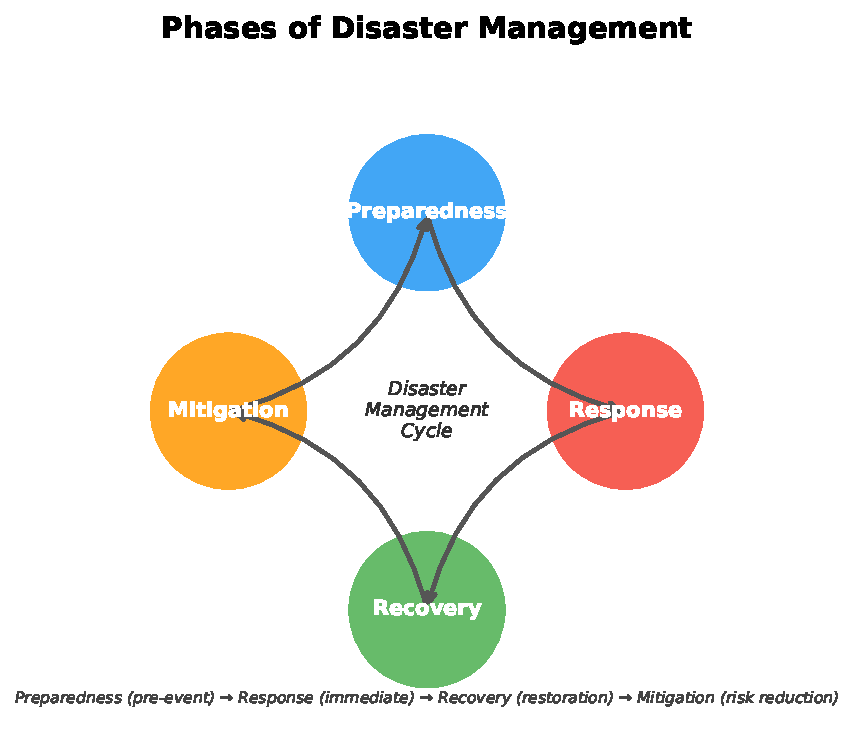
\includegraphics[width=0.62\linewidth]{fig_disaster_phases.pdf}
    \caption{The disaster management cycle.
             Each phase flows into the next, and effective response in
             one phase reduces the burden in subsequent phases.}
  \end{figure}
\end{frame}

% ─────────────────────────────────────────────────────────────
\begin{frame}[allowframebreaks]{14.2.1 --- Preparedness Phase}
  The \textbf{preparedness phase} occurs \emph{before} a disaster strikes.
  Although it may seem paradoxical to plan for an event that has not yet
  happened, pre-disaster planning is the most cost-effective investment
  in disaster response.

  \medskip
  Key preparedness activities that involve routing and location decisions:
  \begin{enumerate}
    \item \textbf{Pre-positioning of supplies}: Deciding which warehouses
          to open and how much stock to store at each, so that supplies
          can be dispatched quickly after an event.
    \item \textbf{Facility location}: Choosing the sites for depots,
          staging areas, and distribution centres in a way that
          minimises expected response time after a disaster.
    \item \textbf{Route planning}: Identifying primary and contingency
          delivery routes in advance, before roads become blocked.
    \item \textbf{Demand estimation}: Using historical data and
          risk models to estimate the quantity of supplies that
          different communities will need in different disaster scenarios.
  \end{enumerate}

  \framebreak

  \begin{block}{Mathematical Models in Preparedness}
    Preparedness is typically modelled as a \textbf{stochastic
    facility-location problem}. Let:
    \begin{itemize}
      \item $I$ be the set of candidate warehouse sites,
      \item $J$ be the set of demand locations (communities at risk),
      \item $S$ be the set of disaster scenarios (earthquake, flood, etc.),
      \item $p_s$ (p sub s) be the probability of scenario $s$ occurring,
      \item $d_{js}$ (d sub j s) be the demand at location $j$ under
            scenario $s$,
      \item $y_i \in \{0,1\}$ (y sub i) be 1 if a warehouse is opened at
            site $i$, 0 otherwise,
      \item $x_{ijs}$ (x sub i j s) be the fraction of demand at $j$ in
            scenario $s$ satisfied from warehouse $i$.
    \end{itemize}

    A basic two-stage stochastic model minimises expected cost:
    \[
      \min \sum_{i \in I} f_i y_i
           + \sum_{s \in S} p_s \sum_{i \in I} \sum_{j \in J}
             c_{ij} d_{js} x_{ijs}
    \]
    where $f_i$ is the fixed cost of opening warehouse $i$, and
    $c_{ij}$ (c sub i j) is the unit transportation cost from $i$ to $j$.
  \end{block}

  \begin{alertblock}{How to Read This Formula}
    The first term $\sum_{i} f_i y_i$ captures the fixed cost of building
    and maintaining warehouses --- you pay this cost before the disaster.
    The second term is the \emph{expected} delivery cost across all
    possible disaster scenarios, weighted by the probability $p_s$ of
    each scenario.
    The model is balancing \textbf{up-front investment} (more warehouses
    = higher fixed cost but shorter delivery distances) against
    \textbf{expected response cost}.
  \end{alertblock}

  \framebreak

  \begin{block}{Pre-Positioning Models (Balcik and Beamon, 2008)}
    Balcik and Beamon model pre-positioning as a
    \emph{maximal covering location problem}: choose depot locations
    and stock levels to maximise the fraction of the at-risk population
    that can be served within a given time threshold $T$.

    Formally, a location $j$ is \emph{covered} if there exists a depot
    $i$ such that the travel time $t_{ij} \leq T$.
    The objective is:
    \[
      \max \sum_{j \in J} w_j z_j
    \]
    subject to: $z_j \leq \sum_{i \in I} a_{ij} y_i$ for all $j$,
    where $w_j$ is the population weight of community $j$,
    $z_j = 1$ if community $j$ is covered, and
    $a_{ij} = 1$ if depot $i$ can reach $j$ within time $T$.
  \end{block}

  The key insight here is that \textbf{the value of a depot is determined
  not just by its own location but by the set of communities it can
  reach within the critical response time window}.
  A depot placed in a central location may cover many communities;
  one placed on a remote island may cover only itself.

  \medskip
  Mete and Zabinsky (2010) extend this to a two-stage stochastic programme
  where the first stage locates and stocks warehouses, and the second stage
  routes vehicles after a disaster is observed.
\end{frame}

% ─────────────────────────────────────────────────────────────
\begin{frame}[allowframebreaks]{14.2.2 --- Response Phase}
  The \textbf{response phase} begins immediately after a disaster and
  typically lasts from a few days to a few weeks.
  This is the most time-critical phase: the first 72 hours after an
  event are especially important because survival rates for trapped or
  injured individuals decline sharply with time.

  \medskip
  \begin{block}{What the Response Phase Demands}
    \begin{itemize}
      \item \textbf{Rapid assessment}: Determine which communities are
            affected and what supplies they need --- often with incomplete
            or contradictory information.
      \item \textbf{Immediate routing}: Deploy vehicles as soon as possible,
            even if demand is not fully known.
      \item \textbf{Dynamic re-routing}: As new information arrives (road
            closures, updated demand figures), routes must be revised.
      \item \textbf{Coordination among agencies}: Multiple aid
            organisations (NGOs, government, military) may operate
            simultaneously, requiring coordination to avoid duplication
            and gaps.
    \end{itemize}
  \end{block}

  \framebreak

  \begin{block}{Response Phase VRP Challenges}
    The response phase maps naturally to a \textbf{dynamic VRP} (DVRP).
    In a DVRP, information about demand, network conditions, and vehicle
    status is revealed over time, and the routing plan must be updated
    in real time.

    Key modelling elements in response-phase VRPs:
    \begin{itemize}
      \item \textbf{One mean of research} (Van Wassenhove, 2006) focuses
            on the logistics response to promote population welfare
            by considering the demand for essentials.
      \item The number of locations $|V|$ may be unknown at the start and
            grows as damage assessment teams report new affected areas.
      \item Road network $G = (V, E)$ changes dynamically as debris is
            cleared or new blockages are discovered.
      \item Vehicle availability fluctuates as vehicles break down,
            run out of fuel, or are commandeered for rescue operations.
    \end{itemize}
  \end{block}

  \medskip
  One important sub-problem in the response phase is
  \textbf{vehicle scheduling with periodic resupply}.
  A vehicle that runs out of supplies must return to a depot to reload,
  creating a natural ``split'' in its route.
  This is modelled as a \textbf{multi-trip VRP}, where each vehicle
  may complete multiple tours before the day ends.

  \framebreak

  \begin{figure}[h]
    \centering
    
\includegraphics[width=0.68\linewidth]{fig_network_flow.pdf}
    \caption{A network flow representation of the response phase.
             The depot (blue square) dispatches vehicles along routes
             to demand locations (coloured circles).
             Vehicle~1 (blue) serves the northern zone;
             Vehicle~2 (red) serves the southern zone.}
  \end{figure}

  \begin{alertblock}{Key Insight: Speed vs.\ Optimality}
    In the response phase, \textbf{a good plan executed quickly
    is better than a perfect plan executed late}.
    This is why fast heuristics (greedy insertion, nearest-neighbour)
    are often preferred over exact optimisation methods during the
    first hours of a disaster response.
  \end{alertblock}
\end{frame}

% ─────────────────────────────────────────────────────────────
\begin{frame}[allowframebreaks]{14.2.3 --- Recovery Phase}
  The \textbf{recovery phase} begins when the immediate crisis has
  stabilised --- the injured have been evacuated, basic supplies have
  been delivered, and the focus shifts to sustaining affected communities
  as they rebuild.

  \medskip
  Although the urgency of the response phase has passed, the recovery
  phase presents its own routing challenges:
  \begin{itemize}
    \item \textbf{Long duration}: Recovery may continue for months or
          years, requiring a \emph{sustainable} supply plan, not just
          an emergency burst of deliveries.
    \item \textbf{Larger and more stable demand}: As population
          concentrations in temporary shelters stabilise, demand becomes
          more predictable --- closer to a classical CVRP (Capacitated VRP).
    \item \textbf{Evolving network}: Roads are gradually repaired, and
          routes that were impassable during the response phase may
          reopen during recovery.
    \item \textbf{Transitioning to commercial logistics}: As conditions
          normalise, emergency logistics are gradually handed over to
          commercial operators.
  \end{itemize}

  \framebreak

  \begin{block}{Recovery Phase Optimisation}
    Recovery phase routing is more amenable to classical VRP methods
    because demand is better known and the network is more stable.
    Models in this phase typically include:
    \begin{itemize}
      \item \textbf{Periodic VRP (PVRP)}: Deliveries are made on a
            fixed schedule (e.g., every three days), and routes are
            optimised for the entire schedule period.
      \item \textbf{Inventory routing}: Vehicles decide both \emph{when}
            and \emph{how much} to deliver to each location, balancing
            delivery frequency against inventory holding costs.
      \item \textbf{Location-routing}: Decisions about which distribution
            points remain open are combined with route optimisation.
    \end{itemize}
  \end{block}

  \medskip
  An important consideration in the recovery phase is
  \textbf{equity of service}.
  As the immediate life-threatening urgency fades, decision-makers
  must ensure that aid reaches \emph{all} affected communities fairly,
  not just those that are easiest to access.
  This motivates a shift from time-minimisation objectives (response phase)
  toward equity-maximisation or balanced-service objectives (recovery phase).

  \begin{alertblock}{Key Insight}
    The recovery phase teaches us that \textbf{routing objectives must
    adapt to the phase of the disaster}.
    The same delivery network may need to switch from
    ``minimise maximum arrival time'' (response) to
    ``minimise standard deviation of service levels'' (recovery)
    as the operation evolves.
  \end{alertblock}
\end{frame}

% =============================================================
\section{Performance Metrics in Disaster Operations}
% =============================================================

\begin{frame}[allowframebreaks]{14.3 --- Performance Metrics in Disaster Operations}
  Measuring the effectiveness of a disaster relief routing plan is
  fundamentally different from evaluating commercial routing.
  In commercial logistics, cost and distance are clear, universal metrics.
  In humanitarian settings, the relevant metrics reflect human welfare,
  which is harder to quantify but no less important.

  \medskip
  The authors identify three principal families of performance metrics
  used in the disaster relief VRP literature:
  \begin{enumerate}
    \item \textbf{Response time}: How quickly does aid arrive?
    \item \textbf{Coverage}: What fraction of the affected population
          receives at least some aid?
    \item \textbf{Demand satisfaction / service equity}: Are supplies
          distributed proportionally to need?
  \end{enumerate}

  \medskip
  Table 14.1 (page 417 of the book) surveys 15 key papers in disaster
  relief VRP research and categorises them by the objective functions
  and metrics they use.
  The table reveals a clear trend: early papers focused on minimising
  total cost or distance, while more recent work increasingly incorporates
  time, equity, and multi-objective formulations.
\end{frame}

% ─────────────────────────────────────────────────────────────
\begin{frame}[allowframebreaks]{14.3.1 --- Response Time}
  \textbf{Response time} is the time that elapses between a disaster
  event and the moment when aid reaches an affected location.
  It is the most natural and widely studied metric in disaster relief,
  because the humanitarian impact of delays is starkly clear: in medical
  emergencies, every hour matters.

  \medskip
  \begin{block}{Defining Response Time}
    Let $n$ be the number of demand locations (affected communities),
    $V = \{v_0, v_1, \ldots, v_n\}$ the set of nodes (with $v_0$ the depot),
    and $t_{ij}$ (t sub i j) the travel time from node $i$ to node $j$.
    For a route $r = (v_0, v_{i_1}, v_{i_2}, \ldots, v_{i_k}, v_0)$,
    the \textbf{arrival time} at the $m$-th location on the route is:
    \[
      a_m = \sum_{\ell=1}^{m} t_{i_{\ell-1}, i_\ell}
    \]
    (a sub m equals the cumulative travel time from the depot through
    the first $m$ stops).
    Here $t_{i_0, i_1}$ is the travel time from the depot to the first stop.
  \end{block}

  \begin{alertblock}{How to Read This Formula}
    $a_m$ accumulates travel times along the route: to reach the third
    stop, you sum the depot-to-stop-1, stop-1-to-stop-2, and
    stop-2-to-stop-3 travel times.
    A longer route, or a route that visits unimportant stops before
    important ones, increases $a_m$ for the later stops.
    This is why route \emph{order} matters so much in disaster settings.
  \end{alertblock}

  \framebreak

  \textbf{Minimising the maximum arrival time} (min-max objective)
  is a common formulation. This ensures that no single community is
  left without aid for too long:
  \[
    \min_{\text{routes}} \max_{j \in V \setminus \{v_0\}} a_j
  \]
  (minimise, over all routing plans, the latest arrival time among
  all demand locations).

  \medskip
  Alternatively, one may minimise the \textbf{sum of arrival times}
  (also called the minimum latency problem):
  \[
    \min \sum_{j \in V \setminus \{v_0\}} a_j
  \]
  This objective gives equal weight to delays at all locations and
  minimises total ``waiting time'' suffered by affected communities.

  \medskip
  \begin{exampleblock}{Worked Example: Comparing Objectives}
    Suppose there are 3 communities with arrival times under two plans:
    \begin{center}
    \begin{tabular}{lccc}
      \toprule
      Plan & $a_1$ & $a_2$ & $a_3$ \\
      \midrule
      A & 30 min & 60 min & 90 min \\
      B & 45 min & 45 min & 60 min \\
      \bottomrule
    \end{tabular}
    \end{center}
    Under \textbf{min-max}: Plan~A scores $\max(30,60,90)=90$;
    Plan~B scores $\max(45,45,60)=60$.
    Plan~B wins.
    Under \textbf{min-sum}: Plan~A scores $30+60+90=180$;
    Plan~B scores $45+45+60=150$.
    Plan~B still wins, but by a different margin.
    Both objectives would choose Plan~B, but in general they can
    select different routes.
  \end{exampleblock}

  \framebreak

  Several papers survey the \textbf{methods for generating solutions
  with good response time}:
  \begin{itemize}
    \item \textbf{Nearest-neighbour heuristics}: Build routes
          greedily by always visiting the closest unvisited location.
          Fast but ignores priorities.
    \item \textbf{Priority-weighted nearest-neighbour}: Modify the
          distance metric to incorporate urgency:
          $d'_{ij} = d_{ij} / w_j$, where $w_j$ (w sub j) is the
          priority weight of location $j$.
          Locations with higher priority are ``pulled closer'' in the
          modified metric, so the heuristic visits them sooner.
    \item \textbf{Time-constrained routing}: Add a hard constraint
          that every location must be served within a maximum time $T$:
          $a_j \leq T$ for all $j$.
  \end{itemize}

  \begin{figure}[h]
    \centering
    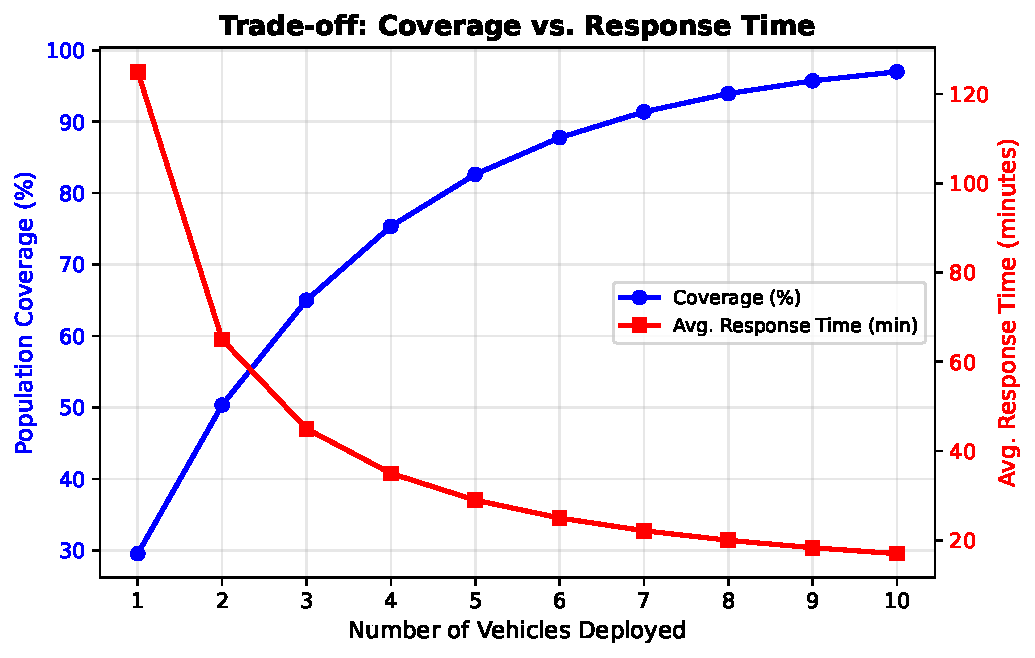
\includegraphics[width=0.65\linewidth]{fig_response_coverage.pdf}
    \caption{Illustrative trade-off between coverage and average
             response time as the number of deployed vehicles increases.
             More vehicles reduce response time but may increase
             coordination complexity and cost.}
  \end{figure}
\end{frame}

% ─────────────────────────────────────────────────────────────
\begin{frame}[allowframebreaks]{14.3.2 --- Coverage}
  \textbf{Coverage} measures the fraction of the affected population
  that receives aid within a specified time window.
  It is a binary or threshold-based concept: a community is either
  ``covered'' (receives aid within time $T$) or ``not covered''.

  \medskip
  \begin{block}{Coverage Formulation}
    Define $z_j = 1$ if demand location $j$ is served within time $T$,
    and $z_j = 0$ otherwise.
    Let $w_j$ (w sub j) be the population weight (or urgency weight)
    of location $j$.
    The \textbf{weighted coverage objective} is:
    \[
      \max \sum_{j \in V} w_j z_j
    \]
    subject to: if location $j$ is served at time $a_j > T$, then
    $z_j = 0$.
  \end{block}

  \begin{alertblock}{How to Read This Formula}
    This says: maximise the total ``weighted population served within
    time $T$.''
    If $w_j$ represents the number of people at location $j$,
    this objective maximises the number of people who receive timely aid.
    It rewards routing decisions that prioritise large, time-critical
    communities --- even if it means leaving small, isolated communities
    unserved.
  \end{alertblock}

  \framebreak

  Coverage objectives are closely related to the classical
  \textbf{Set Covering Problem} and \textbf{Maximum Covering
  Location Problem (MCLP)}, which were developed in the
  facility-location literature and adapted here to routing.

  \medskip
  \begin{exampleblock}{Numerical Coverage Example}
    Suppose 5 communities need aid, with populations:
    $w_1 = 500,\ w_2 = 200,\ w_3 = 800,\ w_4 = 100,\ w_5 = 400$.
    The time threshold is $T = 60$ minutes.
    Two routing plans achieve:
    \begin{center}
    \begin{tabular}{l ccccc c}
      \toprule
      Plan & $a_1$ & $a_2$ & $a_3$ & $a_4$ & $a_5$ & Coverage \\
      \midrule
      A & 30 & 50 & 70 & 40 & 80 & $w_1+w_2+w_4 = 800$ \\
      B & 45 & 65 & 55 & 75 & 50 & $w_1+w_3+w_5 = 1700$ \\
      \bottomrule
    \end{tabular}
    \end{center}
    Plan~B covers communities 1, 3, and 5 (the three largest) within
    60 minutes, achieving a weighted coverage of 1700 vs.\ 800 for
    Plan~A, even though Plan~A covers more communities by count.
    This illustrates why \emph{weighted} coverage is the appropriate
    metric: it aligns with humanitarian goals by prioritising
    the most densely populated areas.
  \end{exampleblock}

  \medskip
  The \textbf{tension between coverage and cost} is inherent:
  achieving 100\% coverage often requires more vehicles and longer
  total travel distances than achieving 80\% coverage.
  In resource-constrained environments, planners must explicitly trade
  off these competing goals.
\end{frame}

% ─────────────────────────────────────────────────────────────
\begin{frame}[allowframebreaks]{14.3.3 --- Demand Satisfaction and Service Equity}
  \textbf{Demand satisfaction} (also called \textbf{service level})
  measures the ratio of supplies delivered to supplies needed at each
  location.
  \textbf{Service equity} is the additional requirement that this ratio
  should be \emph{similar} across all locations --- no community should
  receive disproportionately more or less aid than its needs warrant.

  \medskip
  \begin{block}{Demand Satisfaction Rate}
    Let $d_j$ (d sub j) be the demand (in units of supplies) at
    location $j$, and let $s_j$ (s sub j) be the quantity actually
    delivered.
    The \textbf{demand satisfaction rate} at location $j$ is:
    \[
      \rho_j = \frac{s_j}{d_j} \in [0, 1]
    \]
    where $\rho$ (rho, pronounced ``row'') equals 1 when all demand
    is satisfied, and 0 when nothing is delivered.
    Total demand satisfaction across all locations is:
    \[
      \bar{\rho} = \frac{\sum_{j} s_j}{\sum_{j} d_j}
    \]
    (rho-bar: the overall fraction of total demand that is met).
  \end{block}

  \framebreak

  \begin{block}{Service Equity: The Gini Coefficient and Minimax}
    Two common equity metrics are:
    \begin{enumerate}
      \item \textbf{Minimax satisfaction}: Maximise the minimum
            satisfaction rate across all locations:
            $\max \min_j \rho_j$.
            This ``Rawlsian'' criterion focuses on the worst-off
            community.
      \item \textbf{Minimum variance}: Minimise the variance of
            satisfaction rates:
            $\min \text{Var}(\rho_j) = \min \frac{1}{n}\sum_j (\rho_j - \bar{\rho})^2$.
    \end{enumerate}
    Here $n$ is the number of demand locations, and $\bar{\rho}$ is the
    mean satisfaction rate (rho-bar, the average across all locations).
  \end{block}

  \begin{alertblock}{How to Read Equity Metrics}
    The minimax criterion says: ``the quality of a plan is judged by
    its treatment of the worst-served community.''
    A plan that delivers 100\% to four communities but 0\% to the fifth
    scores 0 on the minimax criterion.
    This is a strong equity requirement that forces balanced distribution.
    The minimum variance criterion is softer: it penalises large
    disparities but does not require all communities to receive the same
    fraction.
  \end{alertblock}

  \framebreak

  \begin{figure}[h]
    \centering
    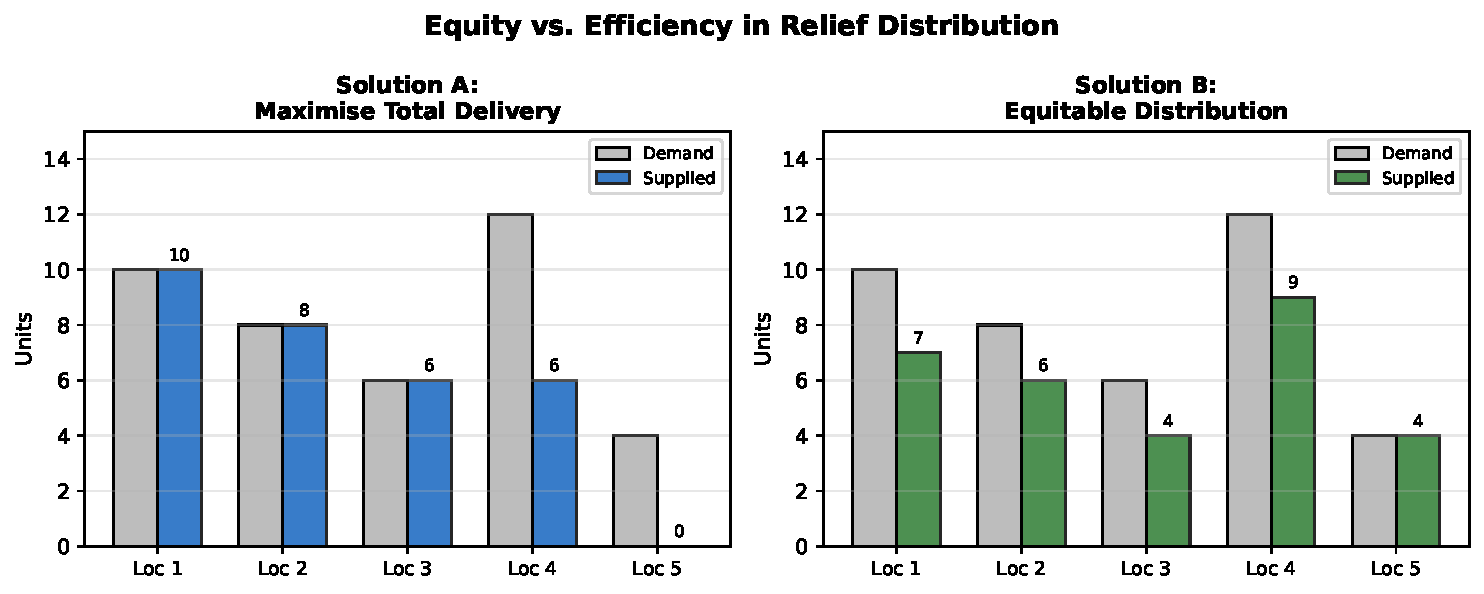
\includegraphics[width=0.75\linewidth]{fig_service_equity.pdf}
    \caption{Left: Solution~A maximises total delivery but leaves
             one community (Loc~5) completely unserved.
             Right: Solution~B distributes supplies proportionally
             to demand, achieving equity at the cost of slightly
             lower total delivery.
             In disaster relief, equity is often mandated by
             humanitarian principles.}
  \end{figure}

  \medskip
  A key paper surveyed by the authors is Huang, Smilowitz, and Balcik
  (2012), which proposes a \textbf{routing problem with equity constraints},
  where each location must receive at least a minimum fraction $\alpha$
  (alpha, the Greek letter for a fraction threshold) of its demand:
  $s_j \geq \alpha \cdot d_j$ for all $j$.
  The objective is then to maximise total delivery subject to this equity
  floor.
\end{frame}

% ─────────────────────────────────────────────────────────────
\begin{frame}[allowframebreaks]{Priority-Weighted Routing: Formal Model}
  One of the most important contributions in the disaster relief VRP
  literature is the introduction of \textbf{location priorities}.
  Not all affected communities have equal urgency: a hospital or a
  community without water may have a far higher priority than a
  community with existing supplies.

  \medskip
  \begin{block}{Local Visiting Priority Model (Nolz, Doerner, Gutjahr, 2010)}
    Each location $j$ is assigned a priority score $p_j > 0$ (p sub j).
    The objective is to \textbf{minimise the priority-weighted sum of
    arrival times}:
    \[
      \min \sum_{j \in V \setminus \{0\}} p_j \cdot a_j
    \]
    where $a_j$ is the arrival time at location $j$ (as defined earlier).
    Locations with high $p_j$ should be visited early in the route,
    since a late arrival at a high-priority location incurs a large
    penalty $p_j \cdot a_j$.
  \end{block}

  \begin{alertblock}{How to Read This Formula}
    This is a weighted sum: each unit of delay at location $j$ costs
    $p_j$ units of penalty.
    If location~A has $p_A = 10$ (critical hospital) and location~B
    has $p_B = 1$ (stable community), delaying A by one hour costs
    10 times as much as delaying B by one hour.
    The optimal route will visit A early, even if it is geographically
    inconvenient, because the priority penalty dominates the distance cost.
  \end{alertblock}

  \framebreak

  \begin{figure}[h]
    \centering
    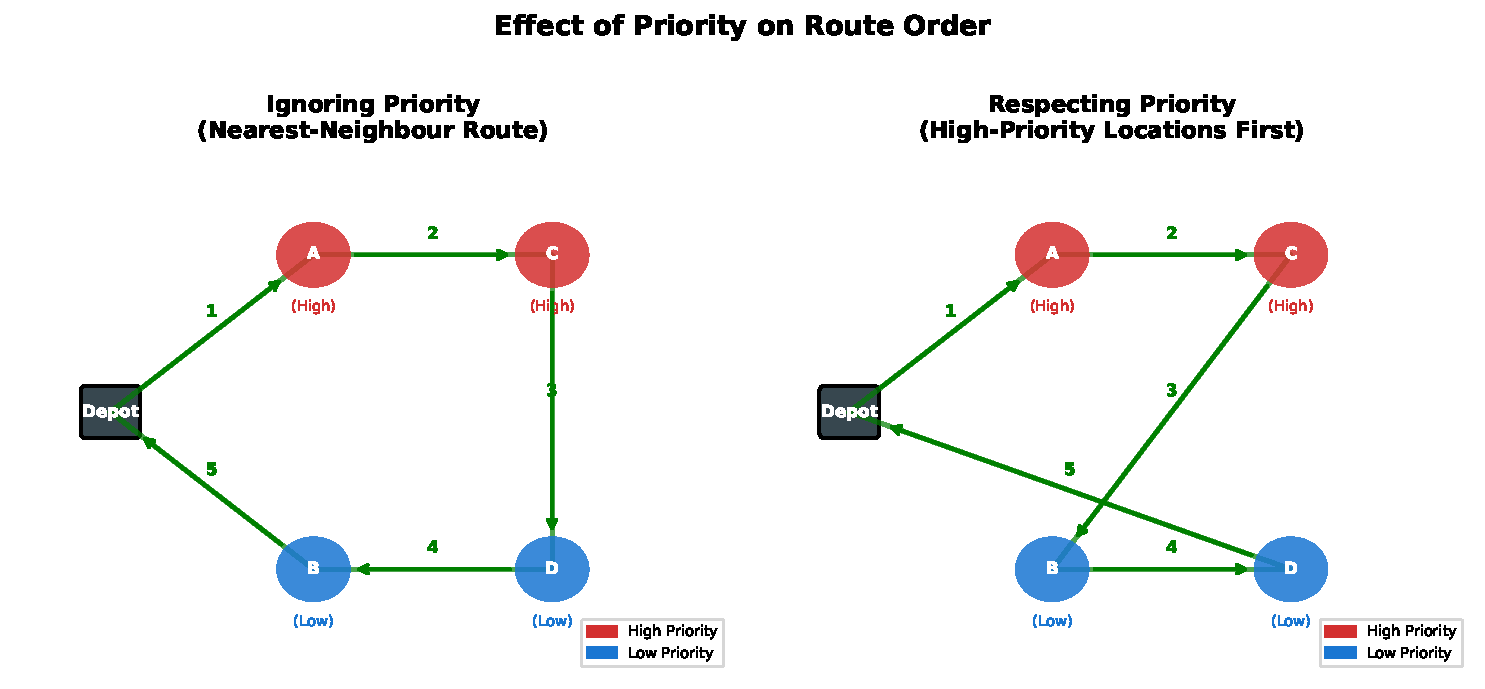
\includegraphics[width=0.75\linewidth]{fig_priority_routing.pdf}
    \caption{Left: A nearest-neighbour route that ignores priorities.
             Right: A priority-aware route that visits high-priority
             locations (red) before low-priority ones (blue),
             even at the cost of a slightly longer total distance.}
  \end{figure}

  \medskip
  The priority-weighted model is related to the classical
  \textbf{Weighted Completion Time Problem} in scheduling theory.
  If we think of each location visit as a ``job'' with weight $p_j$
  and processing time $t_j$ (travel time to reach it), minimising
  $\sum p_j a_j$ is equivalent to scheduling jobs in order of
  decreasing $p_j / t_j$ (the \emph{Smith's Rule} heuristic from
  single-machine scheduling).
  In routing, however, the ``processing times'' are not fixed
  because travel times depend on the order of visits, making
  the problem combinatorially harder.
\end{frame}

% =============================================================
\section{Commercial VRPs vs.\ Disaster Relief VRPs}
% =============================================================

\begin{frame}[allowframebreaks]{14.4 --- Commercial VRPs vs.\ Disaster Relief VRPs}
  The authors devote a section to carefully distinguishing commercial
  VRPs from disaster relief VRPs, because researchers often adapt
  commercial models to humanitarian settings without fully accounting
  for the structural differences.
  Understanding these differences is essential for building models
  that actually help in practice.

  \begin{figure}[h]
    \centering
    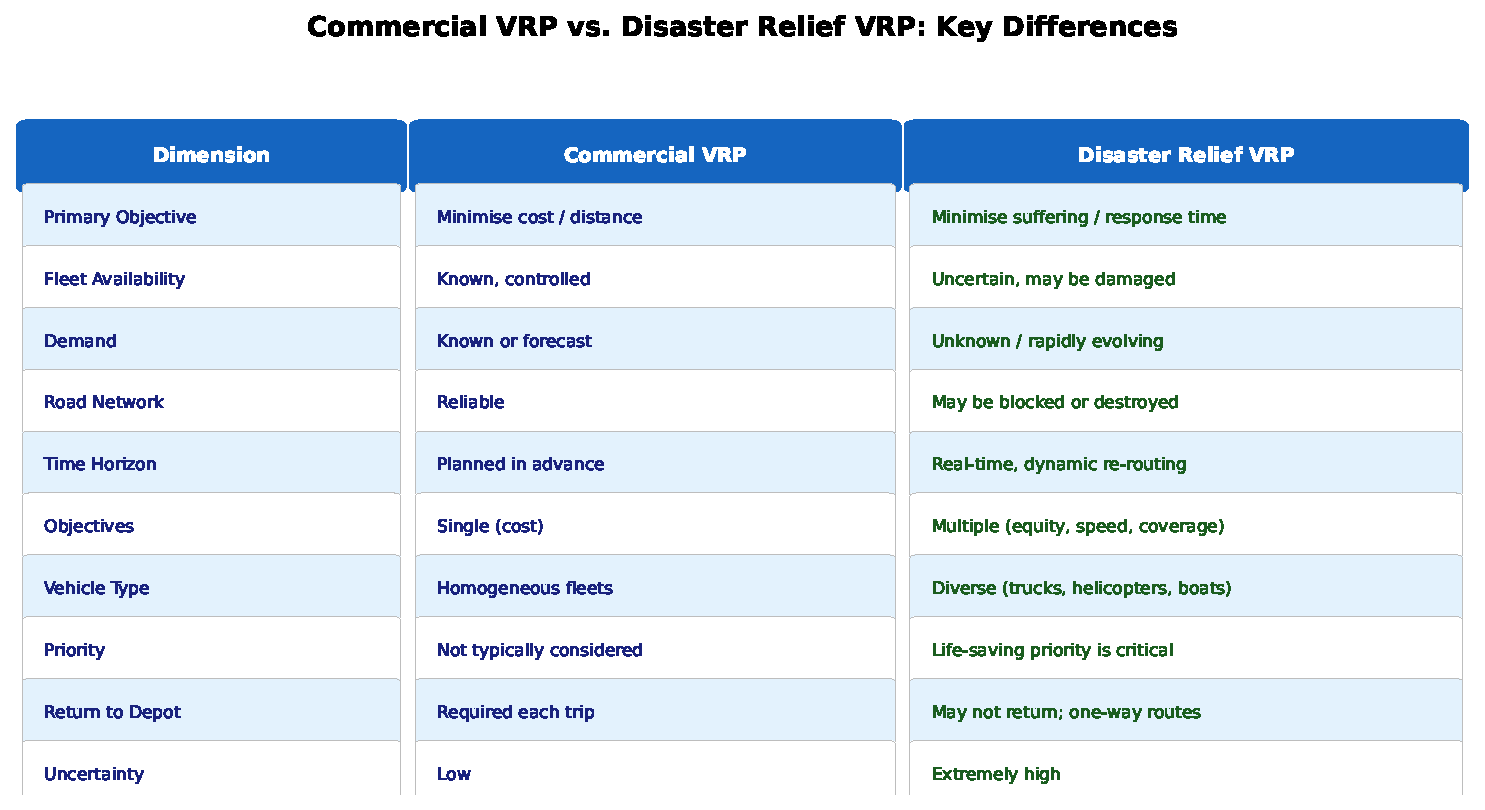
\includegraphics[width=0.90\linewidth]{fig_commercial_vs_disaster.pdf}
    \caption{A systematic comparison of commercial VRP and disaster
             relief VRP across key dimensions.
             Almost every structural assumption of commercial VRP
             must be relaxed or replaced in the humanitarian context.}
  \end{figure}
\end{frame}

% ─────────────────────────────────────────────────────────────
\begin{frame}[allowframebreaks]{14.4.1 --- Low Cost vs.\ Low Arrival Time}
  In commercial logistics, the dominant objective is to
  \textbf{minimise total operating cost}: fuel, driver wages, vehicle
  depreciation.
  Distance is a proxy for cost, so classical VRPs minimise total route
  length.

  \medskip
  In disaster relief, the primary objective is to
  \textbf{minimise arrival time} (response time) or to
  \textbf{maximise welfare} of affected populations.
  Cost matters, but it is subordinate to urgency.

  \medskip
  \begin{block}{A Fundamental Tension: Distance vs.\ Arrival Time}
    The route that minimises \emph{total} travel distance is not
    necessarily the route that minimises \emph{maximum} arrival time.
    Consider a simple example with one vehicle and two locations A and B:
    \begin{itemize}
      \item $d(\text{depot}, A) = 10$, $d(A, B) = 5$, $d(B, \text{depot}) = 12$
      \item Route $(\text{depot} \to A \to B \to \text{depot})$:
            total distance $= 27$, arrival at A = 10, at B = 15.
      \item Route $(\text{depot} \to B \to A \to \text{depot})$:
            total distance $= 27$, arrival at B = 12, at A = 17.
    \end{itemize}
    Both routes have the same total distance, but the first gives
    location A an earlier arrival (10 vs.\ 17).
    If A is more urgent (e.g., a medical emergency), the first route
    is unambiguously better under a humanitarian objective,
    even though the distances are identical.
  \end{block}

  \framebreak

  The mathematical implication is profound.
  Commercial VRP objectives are \textbf{symmetric in customer order}:
  the total distance of a route depends only on which customers are
  on the route, not on the order in which they are visited (given a
  fixed set of customers, TSP-optimal ordering minimises total distance).

  \medskip
  Disaster relief objectives are \textbf{order-sensitive}:
  the same set of locations, visited in a different order, can give
  dramatically different arrival times and thus different humanitarian
  impact.

  \medskip
  \begin{alertblock}{Key Insight}
    This order-sensitivity means that \textbf{classical VRP solvers,
    which optimise insertion order primarily for distance, are poorly
    suited to disaster relief without modification}.
    Algorithms must explicitly account for arrival-time objectives
    and priority constraints.
  \end{alertblock}

  \medskip
  Campbell, VanderBerg, and Werneck (2008) formalised this observation
  by studying the \textbf{deliveries with time windows} variant of
  disaster VRP, showing that even a small change in arrival-time
  objective leads to substantially different optimal routes.
\end{frame}

% ─────────────────────────────────────────────────────────────
\begin{frame}[allowframebreaks]{14.4.2 --- Multiple Objectives and Fleet Considerations}
  \textbf{Commercial VRPs} almost always optimise a single objective
  (usually cost or distance).
  Even when multiple objectives are mentioned, they are typically
  reduced to a single weighted sum.

  \medskip
  \textbf{Disaster relief VRPs} inherently involve multiple, often
  conflicting objectives:
  \begin{enumerate}
    \item Minimise total distance (resource efficiency)
    \item Minimise maximum arrival time (urgency)
    \item Maximise coverage (reach)
    \item Maximise equity (fairness)
    \item Minimise unsatisfied demand (total welfare)
  \end{enumerate}
  These objectives cannot generally be reduced to a single scalar
  without losing important information.
  Multi-objective optimisation methods --- including
  \textbf{Pareto frontier} analysis and \textbf{goal programming} ---
  are therefore more appropriate.

  \medskip
  \begin{block}{Pareto Optimality in Disaster Routing}
    A solution $x^*$ is \textbf{Pareto optimal} if there is no other
    feasible solution $x$ that is at least as good on all objectives
    and strictly better on at least one.
    The set of all Pareto-optimal solutions is called the
    \textbf{Pareto frontier} (or Pareto front).
    Decision-makers can then choose from the Pareto frontier based on
    their preferences, rather than having a single ``optimal'' answer
    imposed on them.
  \end{block}

  \framebreak

  \textbf{Fleet heterogeneity} is another key difference.
  Commercial fleets are typically homogeneous: all vehicles have the
  same capacity and speed.
  Disaster relief may require a mix of:
  \begin{itemize}
    \item \textbf{Trucks}: High capacity, limited to passable roads.
    \item \textbf{Helicopters}: Can reach inaccessible areas but
          have lower capacity and high operating costs.
    \item \textbf{Boats}: Required when roads are flooded.
    \item \textbf{Pack animals}: Used in remote mountain terrain.
  \end{itemize}
  This heterogeneity requires a \textbf{mixed fleet VRP}, where
  each vehicle type has different parameters $(Q_k, v_k, c_k)$:
  capacity $Q_k$ (Q sub k), speed $v_k$ (v sub k), cost per unit
  distance $c_k$ (c sub k).

  \medskip
  Additionally, vehicle availability itself may be uncertain:
  a truck may break down, a helicopter may be requisitioned by
  the military.
  Robust routing models account for this by building contingency
  plans or by formulating stochastic programmes over vehicle
  availability scenarios.
\end{frame}

% ─────────────────────────────────────────────────────────────
\begin{frame}[allowframebreaks]{14.4.3 --- The Min-Max Tour Length Problem}
  One particularly important problem that arises in disaster relief
  (but rarely in commercial logistics) is the
  \textbf{Min-Max VRP}, also called the \textbf{Minimax VRP}:
  minimise the length of the longest route among all vehicles.

  \medskip
  This objective emerges naturally in two situations:
  \begin{enumerate}
    \item \textbf{Time-to-completion}: If all vehicles must finish
          before the next re-supply cycle, the cycle time is
          determined by the \emph{slowest} vehicle (the longest route).
          Minimising the longest route minimises the total cycle time.
    \item \textbf{Workload balance}: Fairness to drivers or
          logistics teams requires that no single vehicle is
          dramatically overloaded relative to others.
  \end{enumerate}

  \begin{figure}[h]
    \centering
    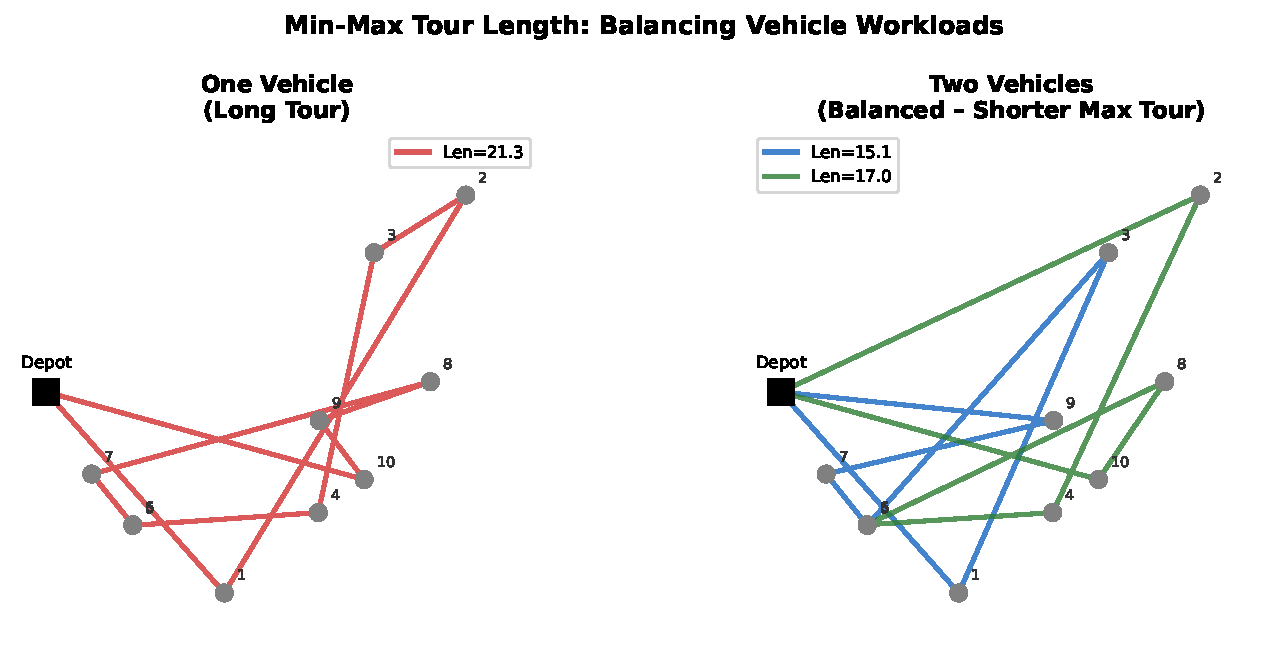
\includegraphics[width=0.72\linewidth]{fig_minmax_tour.pdf}
    \caption{Left: One vehicle completes a very long tour.
             Right: Two balanced vehicles each complete shorter tours.
             The min-max objective drives the planner to choose the
             balanced solution even if it uses more total distance.}
  \end{figure}

  \framebreak

  \begin{block}{Formal Min-Max VRP Model}
    Let $K$ be the number of vehicles and $R_k$ (R sub k) the route
    assigned to vehicle $k$.
    Let $L(R_k)$ denote the length (total distance or time) of route $R_k$.
    The \textbf{Min-Max VRP} minimises:
    \[
      \min \max_{k=1,\ldots,K} L(R_k)
    \]
    subject to standard VRP constraints (all demand locations visited
    exactly once, capacity constraints, etc.).
  \end{block}

  \begin{alertblock}{Why This is Harder Than Minimising Total Distance}
    The min-sum objective (total distance) is a linear function of
    routing decisions, which makes it well-suited for linear programming
    relaxations.
    The min-max objective is a \emph{nonlinear} (piecewise linear)
    function: it equals the largest of the route lengths.
    This can be linearised by introducing an auxiliary variable
    $z \geq L(R_k)$ for all $k$ and minimising $z$, but it substantially
    increases the complexity of the model.
  \end{alertblock}

  \medskip
  Empirical results from Borr\`as and Pastor (2002) and
  Huang, Smilowitz, and Balcik (2012) show that
  \textbf{min-max solutions can be 15--30\% longer in total distance}
  than min-sum solutions, but they reduce the maximum route length
  (and thus the total operation time) by 20--40\%.
  In disaster relief, this trade-off is typically worth making.
\end{frame}

% =============================================================
\section{VRP Models for Disaster Relief}
% =============================================================

\begin{frame}[allowframebreaks]{14.5 --- VRP Models for Disaster Relief: Overview}
  The chapter surveys two main categories of VRP models for disaster
  relief:
  \begin{enumerate}
    \item \textbf{Distribution of relief supplies}: Getting food, water,
          medicine, and shelter materials from depots to affected
          communities.
    \item \textbf{Evacuation routing}: Moving vulnerable people
          (injured, elderly, disabled) from danger zones to safety.
  \end{enumerate}

  \medskip
  Within each category, models range from classical VRP extensions
  (adding priority or equity constraints to the standard CVRP) to
  highly specialised formulations designed for specific disaster types.

  \medskip
  \begin{block}{Common Modelling Elements}
    Across all disaster relief VRP models, the following elements
    appear repeatedly:
    \begin{itemize}
      \item \textbf{Graph} $G = (V, E)$ where $V$ is the set of nodes
            (depot + demand locations) and $E$ is the set of edges
            (road segments).
      \item \textbf{Vehicle fleet} $K = \{1, \ldots, m\}$ with
            capacities $Q_k$ and speeds $v_k$.
      \item \textbf{Demand} $d_j$ at each location $j \in V \setminus \{0\}$.
      \item \textbf{Priority} $p_j$ or urgency weight $w_j$ for each
            demand location.
      \item \textbf{Time windows} $[e_j, l_j]$ (earliest and latest
            acceptable arrival times) in some models.
    \end{itemize}
  \end{block}
\end{frame}

% ─────────────────────────────────────────────────────────────
\begin{frame}[allowframebreaks]{14.5.1 --- Distribution of Relief Supplies: Demand Satisfaction Models}
  The most fundamental disaster relief routing problem asks:
  \textbf{given limited vehicle capacity and a damaged road network,
  how should vehicles route to deliver the maximum possible supplies
  to affected communities?}

  \medskip
  \begin{block}{Basic Capacitated VRP for Relief Distribution}
    Let the node set be $V = \{0, 1, \ldots, n\}$ where node $0$ is
    the depot and nodes $1, \ldots, n$ are demand locations.
    Let $x_{ijk} \in \{0,1\}$ (x sub i j k) = 1 if vehicle $k$ travels
    directly from node $i$ to node $j$.
    Let $y_{jk} \in \{0,1\}$ (y sub j k) = 1 if location $j$ is served
    by vehicle $k$.
    Let $s_{jk} \geq 0$ (s sub j k) be the quantity delivered to
    location $j$ by vehicle $k$.

    \textbf{Objective}: Maximise total demand satisfaction:
    \[
      \max \sum_{k \in K} \sum_{j=1}^{n} s_{jk}
    \]

    \textbf{Subject to}:
    \begin{align}
      & \sum_{k \in K} \sum_{j=1}^{n} s_{jk} \leq D
        \quad \text{(total supply available $D$)} \\
      & \sum_{k \in K} s_{jk} \leq d_j \quad \forall j
        \quad \text{(do not exceed demand)} \\
      & \sum_{j=1}^{n} s_{jk} \leq Q_k \quad \forall k
        \quad \text{(vehicle capacity)} \\
      & s_{jk} \leq M \cdot y_{jk} \quad \forall j,k
        \quad \text{(supply only if visited)} \\
      & x_{ijk}, y_{jk} \in \{0,1\},\ s_{jk} \geq 0
    \end{align}
  \end{block}

  \framebreak

  \begin{alertblock}{Reading the Constraints}
    Constraint (1) says the total amount delivered across all vehicles
    and locations cannot exceed the total available supply $D$.
    Constraint (2) prevents over-delivery: a location with demand
    $d_j = 50$ units should not receive 60.
    Constraint (3) is the vehicle capacity constraint: each vehicle
    can carry at most $Q_k$ units.
    Constraint (4) links the delivery variable $s_{jk}$ to the routing
    variable $y_{jk}$: if vehicle $k$ does not visit location $j$
    ($y_{jk} = 0$), then no supply is delivered ($s_{jk} = 0$).
    Here $M$ is a large constant (``big-M''), a standard modelling
    device used in integer programming.
  \end{alertblock}

  \medskip
  The above model determines \emph{how much} to deliver to each location.
  To determine the actual routes (which order to visit locations in),
  we need additional routing constraints that link the $x_{ijk}$
  variables into valid routes:
  \begin{align}
    & \sum_{j \in V} x_{0jk} = 1 \quad \forall k
      \quad \text{(each vehicle leaves depot once)} \\
    & \sum_{i \in V} x_{ijk} = \sum_{i \in V} x_{jik} \quad \forall j,k
      \quad \text{(flow conservation at each node)} \\
    & \text{Sub-tour elimination constraints (Miller-Tucker-Zemlin or}
      \text{ DFJ cuts)}
  \end{align}

  \framebreak

  \begin{exampleblock}{Worked Distribution Example}
    Suppose we have 1 vehicle with capacity $Q = 15$ units,
    depot at node~0, and 4 demand locations with demands:
    $d_1 = 8,\ d_2 = 5,\ d_3 = 6,\ d_4 = 4$.
    Total demand = 23 units; vehicle capacity = 15 units.
    Since $15 < 23$, the vehicle \emph{cannot} satisfy all demand.

    Two routing options:
    \begin{center}
    \begin{tabular}{lccccc}
      \toprule
      Route & Stops & Delivered & Unmet & Total time \\
      \midrule
      A & $0 \to 1 \to 2 \to 3 \to 0$ & 15 (fills $d_1,d_2,$ part $d_3$) & 8 & 22 min \\
      B & $0 \to 3 \to 2 \to 1 \to 0$ & 15 (fills $d_3,d_4,$ part $d_1$) & 8 & 18 min \\
      \bottomrule
    \end{tabular}
    \end{center}
    Both routes deliver 15 units (vehicle runs full).
    Route~B is shorter (18 vs.\ 22 min).
    But if location~1 has priority $p_1 = 5$ and location~3 has
    $p_3 = 1$, Route~A delivers to the high-priority location first
    and achieves a lower weighted arrival-time cost.
    The optimal choice depends on whether we weight time or equity.
  \end{exampleblock}
\end{frame}

% ─────────────────────────────────────────────────────────────
\begin{frame}[allowframebreaks]{Team Orienteering Problem for Relief Distribution}
  When not all demand locations can be served within the available time
  or vehicle capacity, the problem becomes one of \textbf{selective routing}:
  choose \emph{which} locations to visit (not just in what order).

  \medskip
  This maps to the \textbf{Team Orienteering Problem (TOP)}, sometimes
  called the \textbf{Multiple Depot Team Orienteering Problem (MDTOP)}.
  The TOP is an extension of the Orienteering Problem, itself derived
  from the sport of orienteering where competitors choose which
  checkpoints to visit to maximise collected points.

  \medskip
  \begin{block}{Team Orienteering Problem (TOP) Formulation}
    Given:
    \begin{itemize}
      \item A set $V$ of nodes (locations), each with a reward $r_j \geq 0$,
      \item $m$ vehicles (``teams''), each with a maximum route length
            (or time budget) $T_{\max}$,
      \item A start depot and end depot (possibly the same).
    \end{itemize}
    Find at most $m$ routes --- one per vehicle --- such that:
    \[
      \max \sum_{k=1}^{m} \sum_{j \in V} r_j \cdot y_{jk}
    \]
    subject to: each route has total length $\leq T_{\max}$,
    each location is visited at most once across all routes,
    and routes start and end at the designated depots.
  \end{block}

  \framebreak

  In disaster relief, the \textbf{reward} $r_j$ at location $j$ is
  typically interpreted as the \textbf{demand} $d_j$ (the benefit
  of delivering to that location), or as a \textbf{priority score}
  combining urgency and demand:
  \[
    r_j = p_j \cdot d_j
  \]
  where $p_j$ (p sub j) is the priority of the location and
  $d_j$ (d sub j) is its demand.
  Locations with high demand \emph{and} high urgency get the highest
  reward and are thus most likely to be selected.

  \medskip
  \begin{figure}[h]
    \centering
    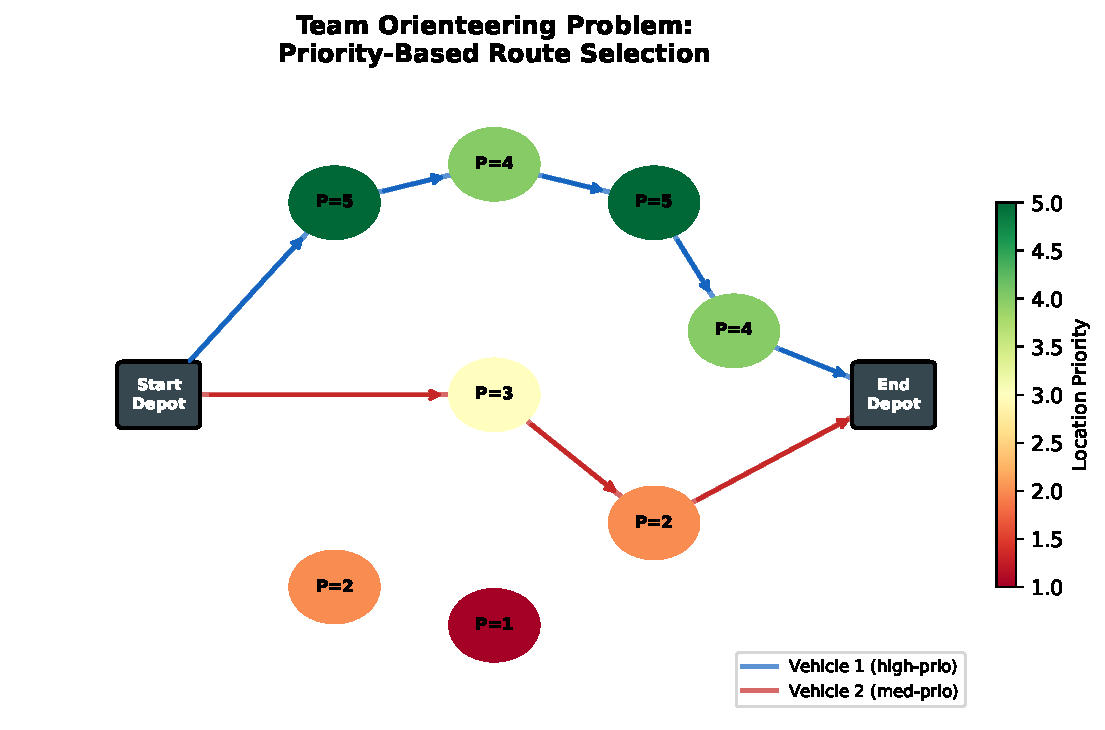
\includegraphics[width=0.68\linewidth]{fig_top_routing.pdf}
    \caption{Team Orienteering Problem routing.
             High-priority locations (green/yellow) are visited first.
             Low-priority locations (red) may be skipped if the time
             budget does not allow their inclusion.
             The colour bar on the right indicates location priority
             from low (red) to high (green).}
  \end{figure}

  \framebreak

  Nolz, Doerner, and Hartl (2010) apply the TOP framework directly
  to disaster relief, with:
  \begin{itemize}
    \item \textbf{Nodes} = affected communities post-disaster
    \item \textbf{Rewards} = population sizes (weighted by urgency)
    \item \textbf{Time budget} = operational day length (e.g., 12 hours)
    \item \textbf{Objective} = maximise total weighted population served
  \end{itemize}
  They solve the problem with a
  \textbf{Variable Neighbourhood Search (VNS)} metaheuristic,
  which iteratively explores neighbourhoods of the current solution
  (by inserting, removing, or swapping location visits) to find
  improvements.

  \medskip
  \begin{block}{Variable Neighbourhood Search (VNS) --- Overview}
    VNS is based on the observation that a local minimum under one
    neighbourhood structure $\mathcal{N}_k$ (N sub k) is not necessarily
    a local minimum under a different neighbourhood structure
    $\mathcal{N}_{k'}$.
    By systematically changing neighbourhood structures, VNS escapes
    local optima that would trap simpler local search methods.
    Algorithm (simplified):
    \begin{enumerate}
      \item Start with an initial feasible solution $x$.
      \item Set $k = 1$ (neighbourhood index).
      \item \textbf{Shake}: Generate a random solution $x'$ in
            $\mathcal{N}_k(x)$ (the $k$-th neighbourhood of $x$).
      \item \textbf{Local search}: Improve $x'$ using a fast local
            search within $\mathcal{N}_1$.
      \item If improved: accept $x'$ as new $x$, reset $k=1$.
      \item Else: increment $k$. If $k > k_{\max}$: stop.
    \end{enumerate}
  \end{block}
\end{frame}

% ─────────────────────────────────────────────────────────────
\begin{frame}[allowframebreaks]{Demand Satisfaction with Route Duration Constraints}
  Raths and Lorenz (2012) study a disaster relief VRP where:
  \begin{itemize}
    \item Vehicles have both capacity constraints \emph{and}
          route duration constraints (a maximum time per route).
    \item Not all demand needs to be satisfied (partial delivery allowed).
    \item The objective is to \textbf{maximise total demand satisfaction}
          subject to feasibility.
  \end{itemize}

  \medskip
  \begin{block}{Raths--Lorenz Model}
    Let $f_j$ (f sub j) be the fraction of demand satisfied at
    location $j$ ($0 \leq f_j \leq 1$).
    The model maximises:
    \[
      \max \sum_{j=1}^{n} w_j \cdot f_j \cdot d_j
    \]
    where $w_j$ (w sub j) is the weight (importance) of location $j$,
    $f_j$ is the fraction delivered, and $d_j$ is the total demand.
    This is equivalent to maximising
    \emph{weighted total units delivered}.
  \end{block}

  \medskip
  The key constraint is that routes must be completed within a
  maximum duration $T$ (e.g., 8 hours per vehicle per day),
  which limits both the number of locations visited and the total
  quantity delivered.

  \framebreak

  \begin{figure}[h]
    \centering
    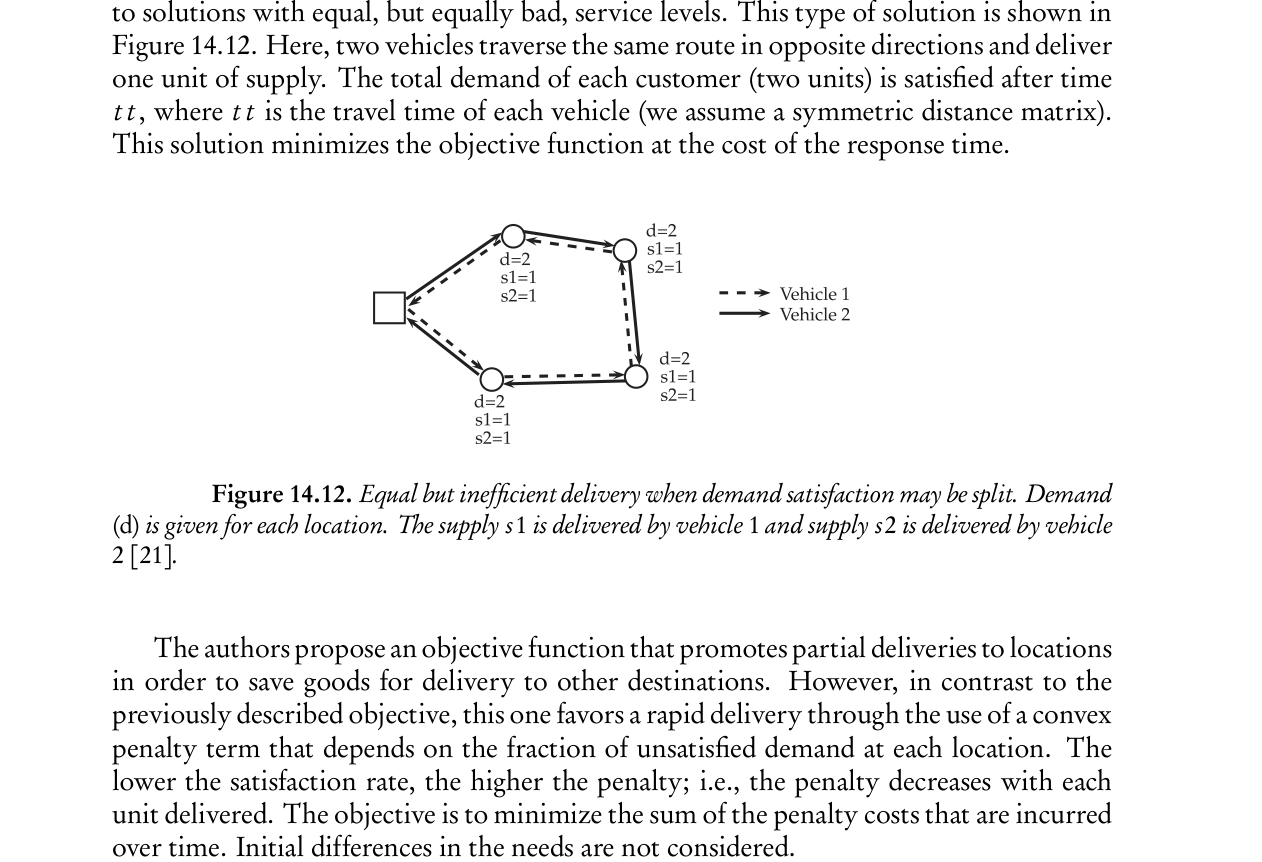
\includegraphics[width=0.72\linewidth]{fig_book_14_10_equity.png}
    \caption{Illustration of balanced supply distribution (from book,
             Figure~14.10).
             The supply allocated to each location depends on
             its distance from the depot and its demand level.}
  \end{figure}

  \begin{alertblock}{Key Trade-off: Time vs.\ Coverage}
    Adding a route duration constraint $\leq T$ means that vehicles
    cannot travel very far, which reduces coverage of distant communities.
    Increasing $T$ expands coverage but may require overnight operations
    or additional fuel stops.
    The model helps decision-makers quantify this trade-off explicitly.
  \end{alertblock}
\end{frame}

% ─────────────────────────────────────────────────────────────
\begin{frame}[allowframebreaks]{Equity-Based Distribution Models}
  Several papers explicitly model \textbf{equity} as a primary objective,
  arguing that in humanitarian contexts, fair distribution is a moral
  imperative, not just a performance metric.

  \medskip
  \begin{block}{Huang, Smilowitz, and Balcik (2012): Routing with Fairness}
    This paper introduces a VRP where the objective is to minimise
    the maximum \textbf{deprivation cost} $\phi_j(a_j)$ (phi sub j
    of a sub j) across all demand locations.
    The deprivation cost is a convex, increasing function of arrival
    time: the longer a community waits, the greater its suffering.

    Specifically:
    \[
      \min \max_{j} \phi_j(a_j)
    \]
    Here $\phi_j(a_j)$ (phi: the Greek letter for a cost function)
    is a location-specific cost function.
    The minimax structure ensures the \emph{worst-served} community
    is improved first, embodying a Rawlsian fairness principle.
  \end{block}

  \begin{alertblock}{How to Read This Formula}
    The formula says: optimise for the community that suffers the most.
    Unlike minimising total cost (which could ignore one very poor
    community to serve many comfortable ones), minimax forces the
    solution to ``raise the floor'' --- improve the worst outcome.
    This is the humanitarian version of the social welfare principle.
  \end{alertblock}

  \framebreak

  \begin{figure}[h]
    \centering
    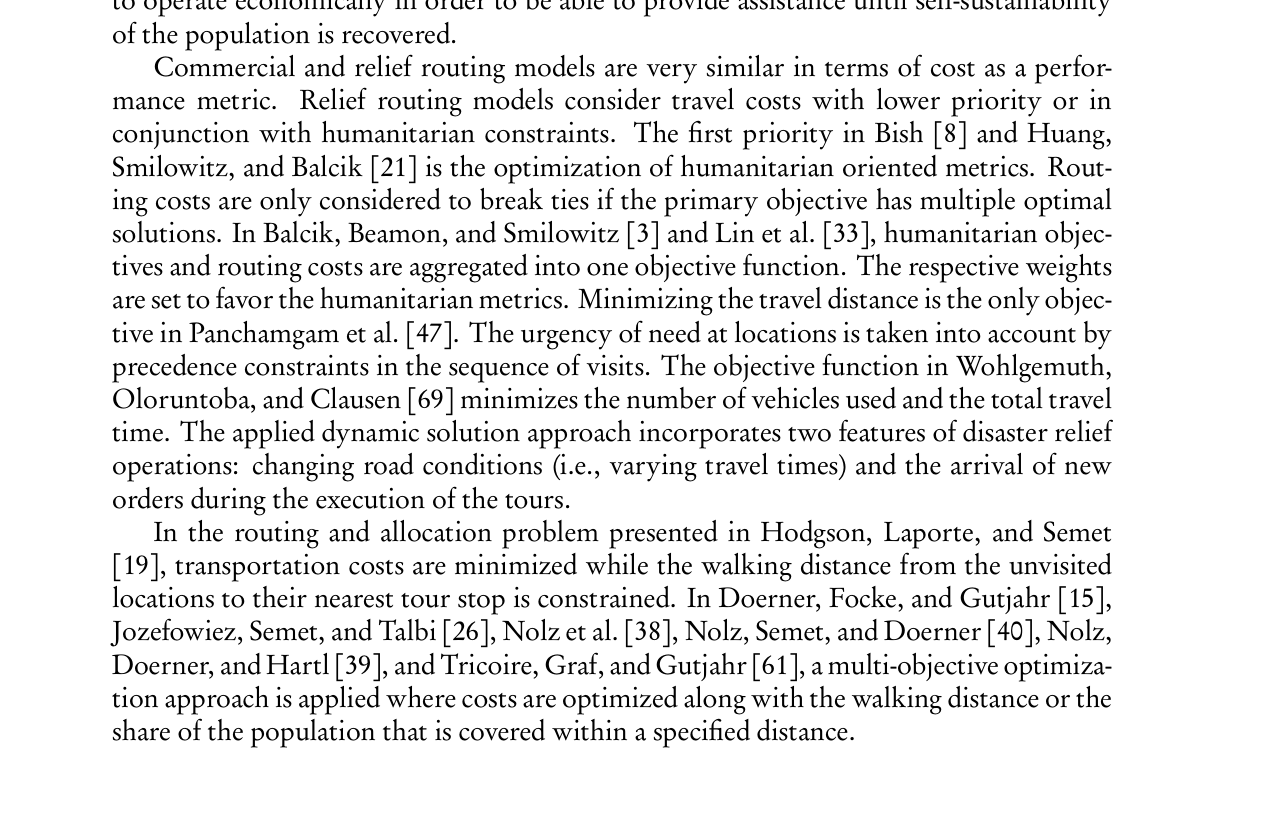
\includegraphics[width=0.75\linewidth]{fig_book_14_11_equity_split.png}
    \caption{Comparing balanced and unbalanced supply distribution
             after applying a wave (from book Figure~14.11).
             In both panels the total supply is the same, but the
             equity metric favours the balanced case.}
  \end{figure}

  \medskip
  Vitoriano, Ortu\~no, and Tirado (2009) propose a
  \textbf{goal programming} approach that treats multiple objectives
  (cost, reliability, equity, and security) simultaneously.
  Goal programming works by setting a \emph{target level} for each
  objective and minimising the weighted sum of deviations from targets.
  This gives decision-makers a structured way to articulate priorities
  and explore trade-offs without collapsing everything into a single
  scalar.
\end{frame}

% ─────────────────────────────────────────────────────────────
\begin{frame}[allowframebreaks]{14.5.2 --- Evacuation Routing}
  \textbf{Evacuation routing} is the second major category of disaster
  relief VRP.
  The goal is to move people --- not goods --- from danger zones to
  safety, using a fleet of vehicles operating on a (possibly damaged)
  road network.

  \medskip
  Evacuation routing has several unique features that distinguish it
  from supply distribution:
  \begin{enumerate}
    \item \textbf{The ``commodity'' is human}: Vehicles transport people
          rather than goods, imposing safety and dignity constraints.
    \item \textbf{One-way flow}: Vehicles go from hazard zones \emph{to}
          shelters; the return trip brings no immediate benefit.
    \item \textbf{Contraflow operations}: Road capacity can be doubled
          by reversing normally inbound lanes to carry outbound
          evacuation traffic.
    \item \textbf{Capacity of shelters}: Shelters have limited capacity;
          routing must account for where evacuees can actually go.
    \item \textbf{Self-evacuation}: Many people evacuate independently
          by car, creating massive traffic congestion that affects
          vehicle routing.
  \end{enumerate}

  \framebreak

  \begin{figure}[h]
    \centering
    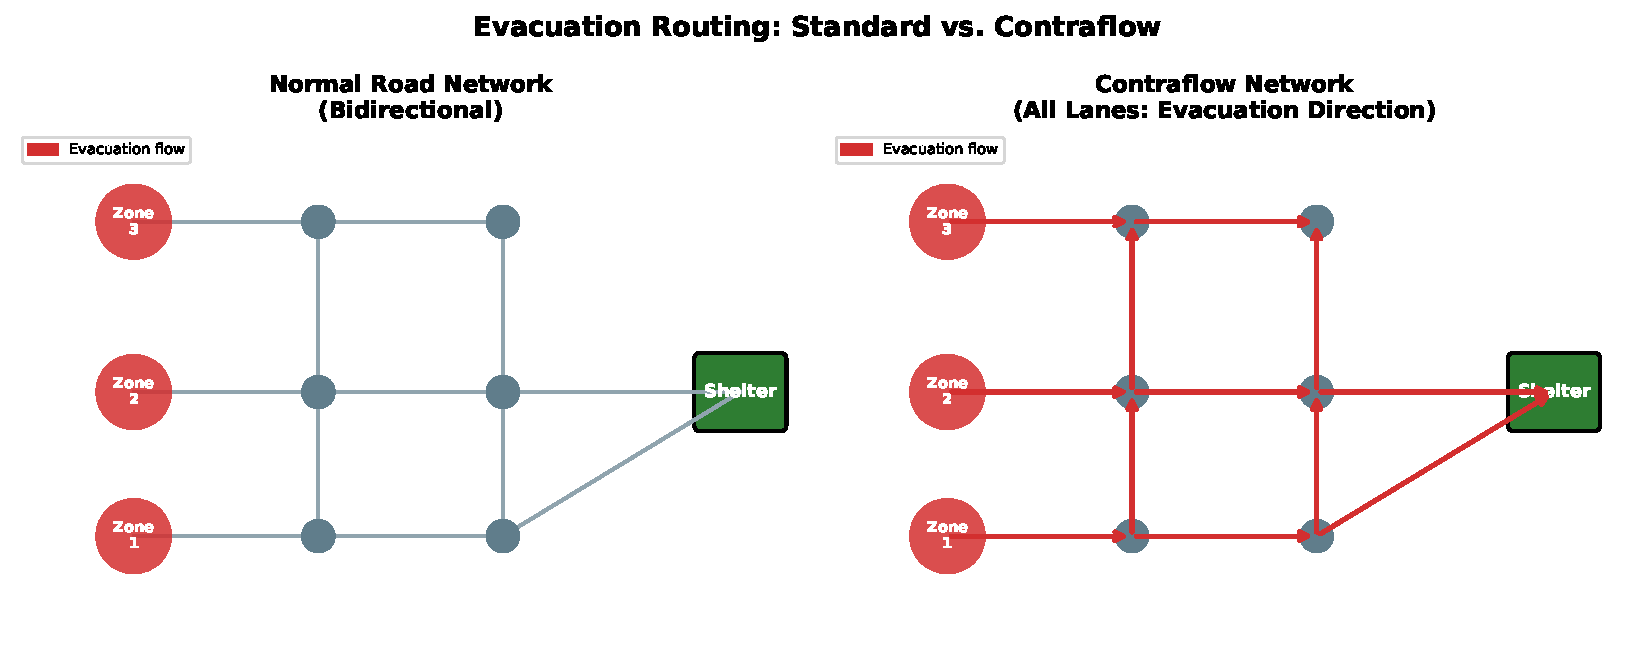
\includegraphics[width=0.80\linewidth]{fig_evacuation_contraflow.pdf}
    \caption{Left: Standard bidirectional road network.
             Right: Contraflow configuration where all lanes are
             re-directed outbound to maximise evacuation throughput.
             Contraflow effectively doubles the capacity of evacuation
             routes but requires coordination with traffic management
             authorities.}
  \end{figure}

  \begin{block}{Network Structure for Evacuation}
    Evacuation is modelled on a directed graph $G = (V, A)$ where
    $V$ is the set of nodes (evacuation zones + shelters + road
    intersections) and $A$ is the set of directed arcs (road segments
    with a specific direction of travel).
    \textbf{Contraflow} is modelled by adding reverse arcs to
    normally one-directional road segments, with appropriate capacity
    and travel time parameters.
  \end{block}
\end{frame}

% ─────────────────────────────────────────────────────────────
\begin{frame}[allowframebreaks]{Evacuation Routing: Key Models}
  \begin{block}{Yi and \"{O}zdamar (2007): Dynamic Logistics Coordination}
    Yi and \"{O}zdamar model evacuation and supply distribution
    \emph{simultaneously} in a multi-period network flow problem.
    In period $t$, vehicles can carry either supplies (inbound to
    disaster zones) or evacuees (outbound to shelters), subject to
    vehicle capacity constraints.

    This is a \textbf{dynamic network flow problem}:
    \begin{itemize}
      \item Nodes represent (location, time) pairs.
      \item Arcs represent vehicle movements or waiting in place.
      \item Flow on each arc is bounded by vehicle capacity.
    \end{itemize}
    The objective balances the urgency of delivering supplies against
    the urgency of evacuating injured people.
  \end{block}

  \medskip
  \begin{block}{Evacuation with Heterogeneous Demand}
    Not all evacuees have the same mobility.
    The \textbf{special needs} population (elderly, disabled, hospitalised)
    cannot self-evacuate and must be given priority access to vehicles.
    Ozbay and Yazici (2006) study the allocation of transit buses
    to special-needs evacuation, formulating it as a VRP where:
    \begin{itemize}
      \item Each bus picks up evacuees from multiple pickup points
            (nursing homes, hospitals) and delivers them to a shelter.
      \item Bus routes are constrained by travel time and vehicle capacity.
      \item The objective is to minimise the number of buses required
            to evacuate all special-needs individuals within
            a time window.
    \end{itemize}
  \end{block}

  \framebreak

  \begin{block}{Contraflow Optimisation (Lim, 2008)}
    Lim models contraflow assignment as an optimisation problem:
    given a set of road segments that \emph{could} be reversed, decide
    which segments to reverse (and at what cost) in order to maximise
    network throughput for evacuation.

    Formally, let $b_e \in \{0,1\}$ (b sub e) = 1 if arc $e$ is
    reversed (contraflow), 0 otherwise.
    The total contraflow capacity on the evacuation corridors is:
    \[
      \text{Throughput} = \sum_{e \in E} \left( c_e + b_e \cdot c_e' \right)
    \]
    where $c_e$ is the original capacity of arc $e$ and $c_e'$
    (c prime sub e) is the additional capacity gained by reversing it.
    The constraint is that implementing contraflow on certain segments
    conflicts with implementing it on adjacent segments
    (you cannot reverse roads in both directions at the same intersection).
  \end{block}

  \medskip
  \begin{alertblock}{Key Insight: Evacuation is a Supply Chain in Reverse}
    While supply distribution moves goods \emph{toward} affected populations,
    evacuation moves people \emph{away} from danger.
    The vehicle routing mathematics is similar, but the priorities,
    constraints, and coordination requirements are different.
    Effective evacuation planning requires routing models to be
    integrated with traffic management, shelter management,
    and public communication systems.
  \end{alertblock}
\end{frame}

% ─────────────────────────────────────────────────────────────
\begin{frame}[allowframebreaks]{Dynamic Routing in Disaster Settings}
  A major distinguishing feature of disaster relief VRP is
  \textbf{dynamism}: both the environment and the information
  available to planners change rapidly during an operation.

  \medskip
  \begin{block}{Dynamic VRP (DVRP) Formulation}
    In a DVRP, the input data $\{d_j, p_j, t_{ij}\}$ (demand,
    priority, travel time) is not fully known at the start of the
    planning horizon.
    New information arrives at discrete time points $\tau_1, \tau_2, \ldots$
    ($\tau$: tau, the Greek letter for time steps).
    At each $\tau_t$, the routing plan is \textbf{re-optimised} based
    on all available information.

    The degree of dynamism $\delta$ (delta, the Greek letter) is defined as:
    \[
      \delta = \frac{\text{Number of requests known only after start}}
                    {\text{Total number of requests}}
    \]
    Commercial DVRP typically has $\delta \approx 0.1$--$0.3$;
    disaster relief DVRP can have $\delta \approx 0.7$--$1.0$,
    meaning most demand is unknown at the start of operations.
  \end{block}

  \framebreak

  \begin{block}{Re-optimisation Strategies}
    When new information arrives (a new affected area is reported,
    a road is found to be blocked), the dispatcher must decide:
    \begin{enumerate}
      \item \textbf{Myopic re-routing}: Immediately update routes
            based on current information, ignoring future uncertainty.
            Simple and fast, but may make poor long-term decisions.
      \item \textbf{Anticipatory re-routing}: Use probabilistic models
            of where future requests are likely to arise and build
            routes that are robust to likely future scenarios.
            More complex but can reduce total response time by 10--20\%.
      \item \textbf{Scenario-based robust routing}: Enumerate a set of
            likely future scenarios and find a routing plan that
            performs well across all of them (a ``hedged'' plan).
    \end{enumerate}
  \end{block}

  \medskip
  Wohlgemuth, Oloruntoba, and Clausen (2012) study
  \textbf{dynamic vehicle routing with anticipation} in disaster relief,
  showing that anticipatory strategies outperform myopic re-routing
  when the disaster evolves predictably (e.g., a flood that advances
  in a known direction).

  \medskip
  \begin{alertblock}{Key Insight}
    The fundamental challenge of dynamic disaster routing is
    \textbf{balancing responsiveness to new information against
    the disruption cost of re-routing vehicles in the field}.
    Constant re-routing may confuse field teams and increase travel
    distances; too little re-routing leads to poor adaptation.
  \end{alertblock}
\end{frame}

% ─────────────────────────────────────────────────────────────
\begin{frame}[fragile]{Python Implementation: Priority-Weighted Greedy Routing}
  The following Python code implements a \textbf{priority-weighted
  nearest-neighbour heuristic} for disaster relief routing.
  The heuristic builds a route by always selecting the unvisited
  location with the best priority-to-distance ratio.

\begin{lstlisting}
import numpy as np

def priority_nn_heuristic(depot, locations, demands, priorities,
                           vehicle_capacity):
    """
    Priority-weighted nearest-neighbour heuristic for disaster VRP.

    Parameters
    ----------
    depot       : (x, y) coordinates of the depot
    locations   : list of (x, y) coordinates of demand locations
    demands     : list of demand values d_j for each location
    priorities  : list of priority weights p_j for each location
    vehicle_capacity : Q (maximum load per vehicle)

    Returns
    -------
    routes : list of routes, each route is a list of location indices
    """
    n = len(locations)
    unvisited = set(range(n))   # indices of unvisited locations
    routes = []                 # list of completed routes

    while unvisited:
        route = []              # current route being built
        load = 0                # current vehicle load
        current = depot         # vehicle starts at depot

        while unvisited:
            # Find the best next location: highest p_j / d(current, j)
            best_score = -1
            best_j = None
            for j in unvisited:
                if load + demands[j] > vehicle_capacity:
                    continue    # skip if capacity exceeded
                dist = np.linalg.norm(
                    np.array(locations[j]) - np.array(current))
                if dist < 1e-9:
                    dist = 1e-9   # avoid division by zero
                score = priorities[j] / dist  # priority per unit distance
                if score > best_score:
                    best_score = score
                    best_j = j

            if best_j is None:
                break   # no feasible location: start a new route

            route.append(best_j)
            load += demands[best_j]
            current = locations[best_j]
            unvisited.remove(best_j)

        routes.append(route)    # vehicle returns to depot

    return routes

# --- Example ---------------------------------------------------
depot     = (0, 0)
locations = [(2,3), (5,1), (3,5), (7,4), (1,6)]
demands   = [4,    5,     3,     6,     2    ]
priorities= [3,    1,     5,     2,     4    ]
capacity  = 10

routes = priority_nn_heuristic(depot, locations, demands,
                               priorities, capacity)
for i, r in enumerate(routes):
    print(f"Vehicle {i+1}: depot -> "
          + " -> ".join(str(j+1) for j in r) + " -> depot")
\end{lstlisting}

  \medskip
  \textbf{Key design choice:} The score $p_j / d(\text{current}, j)$
  rewards high-priority locations and penalises distant locations.
  Increasing $p_j$ ``pulls'' the vehicle toward that location;
  increasing distance ``pushes'' it away.
  This greedy heuristic is $O(n^2)$ per route and very fast in practice.
\end{frame}

% ─────────────────────────────────────────────────────────────
\begin{frame}[fragile]{Python Implementation: Computing Arrival Times and Equity Metrics}
\begin{lstlisting}
import numpy as np

def route_arrival_times(depot, locations, route, speed=1.0):
    """
    Compute arrival times at each stop in a route.

    Parameters
    ----------
    depot     : (x, y) tuple -- starting point
    locations : list of (x, y) tuples for all demand nodes
    route     : list of location indices in visit order
    speed     : vehicle speed (distance units per time unit)

    Returns
    -------
    arrivals : list of arrival times (one per stop in route)
    """
    arrivals = []
    current = np.array(depot)
    time = 0.0
    for j in route:
        dest = np.array(locations[j])
        dist = np.linalg.norm(dest - current)
        time += dist / speed
        arrivals.append(time)
        current = dest
    return arrivals

def demand_satisfaction_rate(demands, delivered):
    """
    Compute per-location satisfaction rate rho_j = s_j / d_j.
    demands   : list of demands d_j
    delivered : list of quantities delivered s_j
    Returns   : list of rho_j values
    """
    return [s / d if d > 0 else 0.0 for s, d in zip(delivered, demands)]

def equity_metrics(rho_list):
    """
    Compute equity metrics for a list of satisfaction rates rho_j.
    Returns: (mean, variance, minimax satisfaction, Gini coefficient)
    """
    rho = np.array(rho_list)
    mean_rho  = np.mean(rho)
    var_rho   = np.var(rho)
    min_rho   = np.min(rho)   # worst-served location (minimax)
    # Gini coefficient: 0 = perfect equity, 1 = perfect inequality
    n = len(rho)
    sorted_rho = np.sort(rho)
    gini = (2 * np.sum((np.arange(1, n+1)) * sorted_rho)
            / (n * np.sum(sorted_rho)) - (n+1)/n) if np.sum(rho) > 0 else 0
    return mean_rho, var_rho, min_rho, gini

# --- Example ---------------------------------------------------
demands   = [10, 8, 6, 12, 4]
delivered = [10, 8, 6,  6, 0]   # Solution A (unequal)
rho = demand_satisfaction_rate(demands, delivered)
print("Satisfaction rates:", [f"{r:.2f}" for r in rho])
mean_r, var_r, min_r, gini = equity_metrics(rho)
print(f"Mean: {mean_r:.2f}, Variance: {var_r:.3f}, "
      f"Minimax: {min_r:.2f}, Gini: {gini:.3f}")
\end{lstlisting}

  The Gini coefficient (a standard economic inequality measure) equals
  0 when all locations receive the same satisfaction rate, and approaches
  1 when one location receives everything and the rest receive nothing.
  In disaster relief, a Gini coefficient below 0.2 is typically
  considered acceptably equitable.
\end{frame}

% =============================================================
\section{Conclusions and Future Research}
% =============================================================

\begin{frame}[allowframebreaks]{14.6 --- Conclusions and Future Research Directions}
  The authors conclude by summarising the state of the disaster relief
  VRP literature and identifying the most important open research questions.

  \medskip
  \begin{block}{Main Conclusions}
    \begin{enumerate}
      \item \textbf{The field is young but growing rapidly.}
            The number of papers on humanitarian logistics and disaster
            relief routing has approximately doubled every five years
            since 2000.
      \item \textbf{Commercial VRP models require substantial modification.}
            Simply applying existing VRP heuristics to disaster data
            produces plans that may be efficient in distance but poor
            in humanitarian terms.
      \item \textbf{Multi-objective formulations are essential.}
            Capturing the trade-offs between speed, equity, and coverage
            requires genuinely multi-objective optimisation, not just
            a weighted single objective.
      \item \textbf{Vehicle routing compatibility matters.}
            Requires that all locations be reachable by at least one
            vehicle type, even if roads are blocked.
      \item \textbf{Dynamic and stochastic elements are unavoidable.}
            Static, deterministic models miss the most important
            operational challenge: responding to rapidly changing
            information.
    \end{enumerate}
  \end{block}

  \framebreak

  \begin{block}{Open Research Directions}
    The authors identify several areas where future research is
    most needed:
    \begin{enumerate}
      \item \textbf{Pre-positioning with network uncertainty.}
            Better models that account for the possibility that specific
            roads or depots will be unavailable after a disaster,
            requiring robust pre-positioning decisions.
      \item \textbf{Integration across phases.}
            Models that span the preparedness--response--recovery
            continuum, rather than treating each phase in isolation.
      \item \textbf{Coordination among multiple agencies.}
            Mechanisms for coordinating routing decisions across NGOs,
            government agencies, and military organisations that may
            have conflicting objectives.
      \item \textbf{Incorporating self-evacuation behaviour.}
            Realistic evacuation models must account for the fact that
            most people evacuate independently, creating congestion that
            affects official vehicle routing.
      \item \textbf{Algorithmic scalability.}
            Disaster-scale instances can involve thousands of locations
            and dozens of vehicles.
            Exact methods are too slow; better large-scale heuristics
            and metaheuristics are needed.
    \end{enumerate}
  \end{block}

  \framebreak

  \begin{block}{Specific Research Gap: Vehicle Routing Compatibility}
    One requirement that the authors flag as insufficiently studied
    is the concept of \textbf{routing compatibility} in disaster VRP.
    In commercial settings, we typically assume that all vehicles can
    reach all customers.
    In disaster settings, this assumption fails: a heavy truck cannot
    traverse a washed-out bridge; a helicopter cannot land in a dense
    urban canyon.

    Future models should explicitly encode an
    \textbf{access compatibility matrix} $A_{kj} \in \{0,1\}$
    (A sub k j) = 1 if vehicle type $k$ can access location $j$,
    0 otherwise.
    This matrix, combined with routing constraints, forces the model
    to assign each location to a compatible vehicle type.
  \end{block}

  \medskip
  \begin{alertblock}{Final Key Insight}
    Disaster relief routing is one of the most socially impactful
    applications of combinatorial optimisation.
    Even modest improvements in routing efficiency --- reducing
    average response time by 20\% or improving supply equity by 30\% ---
    can translate directly into lives saved.
    This makes it both a compelling research area and a responsibility
    for the operations research community.
  \end{alertblock}
\end{frame}

% ─────────────────────────────────────────────────────────────
\begin{frame}[allowframebreaks]{Summary: Key Concepts and Models}
  This frame provides a consolidated reference for the main concepts
  and formulas introduced in this chapter.

  \medskip
  \textbf{Performance Metrics:}
  \begin{itemize}
    \item \textbf{Arrival time} at location $j$:
          $a_j = \sum_{\ell=1}^{m} t_{i_{\ell-1}, i_\ell}$
          (cumulative travel time along the route to location $j$).
    \item \textbf{Min-max response time}: $\min \max_j a_j$
          (minimise the latest arrival).
    \item \textbf{Min-sum response time}: $\min \sum_j a_j$
          (minimise total waiting time).
    \item \textbf{Demand satisfaction rate}:
          $\rho_j = s_j / d_j$ (rho sub j).
    \item \textbf{Service equity}:
          $\min \text{Var}(\rho_j)$ or $\max \min_j \rho_j$.
  \end{itemize}

  \medskip
  \textbf{VRP Variants for Disaster Relief:}
  \begin{itemize}
    \item \textbf{Priority-weighted VRP}: Objective $\min \sum_j p_j a_j$.
    \item \textbf{Team Orienteering Problem (TOP)}: Select which
          locations to visit within a time budget to maximise reward.
    \item \textbf{Min-Max VRP}: $\min \max_k L(R_k)$ (balance workloads).
    \item \textbf{Dynamic VRP (DVRP)}: Real-time re-optimisation as
          information evolves.
    \item \textbf{Stochastic VRP}: Demand $d_j$ is a random variable;
          plan under uncertainty.
  \end{itemize}

  \framebreak

  \textbf{Commercial vs.\ Disaster Relief VRP --- At a Glance:}
  \begin{center}
  \begin{tabular}{p{3.5cm} p{4.5cm} p{4.5cm}}
    \toprule
    \textbf{Dimension} & \textbf{Commercial VRP} & \textbf{Disaster Relief VRP} \\
    \midrule
    Objective & Min cost / distance & Min time; Max equity \\
    Fleet & Homogeneous & Heterogeneous \\
    Demand & Known & Uncertain \\
    Network & Reliable & Disrupted \\
    Time horizon & Planned & Real-time \\
    Priorities & Absent & Life-critical \\
    Return to depot & Required & May not return \\
    \bottomrule
  \end{tabular}
  \end{center}

  \medskip
  \begin{alertblock}{Take-Home Message}
    Vehicle routing in disaster relief is not simply ``standard VRP
    with a different dataset.''
    The objectives, constraints, and operational environment are
    fundamentally different.
    Effective humanitarian logistics requires purpose-built VRP models
    that encode urgency, equity, uncertainty, and multi-vehicle
    coordination --- and algorithms fast enough to be useful
    in the hours immediately following a disaster.
  \end{alertblock}
\end{frame}

% ─────────────────────────────────────────────────────────────
\begin{frame}[allowframebreaks]{Selected Bibliography}
  The following key references from the chapter are listed here for
  the reader's convenience.
  They represent the most important works cited in the survey.

  \medskip
  \begin{enumerate}\setlength{\itemsep}{3pt}\footnotesize
    \item B.\ Balcik and B.M.\ Beamon,
          \textit{Facility location in humanitarian relief},
          International Journal of Logistics, 11 (2008), pp.\ 101--121.
    \item A.\ Campbell, L.\ VanderBerg, and R.\ Werneck,
          \textit{Optimising humanitarian logistics},
          Transportation Science, 42 (2008), pp.\ 330--348.
    \item T.G.\ Crainic, N.\ Ricciardi, and G.\ Storchi,
          \textit{Models for evaluating and planning city logistics systems},
          Transportation Science, 43 (2009), pp.\ 432--454.
    \item M.\ Huang, K.\ Smilowitz, and B.\ Balcik,
          \textit{A continuous approximation approach for assessment routing in disaster relief},
          Transportation Research Part B, 46 (2012), pp.\ 997--1016.
    \item L.\ Ozbay and A.\ Yazici,
          \textit{Evacuation transportation planning},
          Transportation Research Record, (2006).
    \item P.\ Nolz, F.\ Doerner, and R.\ Hartl,
          \textit{Water distribution in disaster relief},
          International Journal of Physical Distribution, 40 (2010), pp.\ 693--708.
    \item J.\ Raths and D.\ Lorenz,
          \textit{Routing for demand satisfaction in humanitarian logistics},
          Computers and Operations Research, 39 (2012), pp.\ 808--822.
    \item B.\ Vitoriano, T.\ Ortu\~no, and G.\ Tirado,
          \textit{HADS, a goal programming-based humanitarian aid distribution system},
          Journal of Multi-Criteria Decision Analysis, 16 (2009), pp.\ 55--64.
    \item S.\ Wohlgemuth, R.\ Oloruntoba, and U.\ Clausen,
          \textit{Dynamic vehicle routing with anticipation in disaster relief},
          Socio-Economic Planning Sciences, 46 (2012), pp.\ 261--271.
    \item W.\ Yi and L.\ \"{O}zdamar,
          \textit{A dynamic logistics coordination model for evacuation and support in disaster response},
          European Journal of Operational Research, 179 (2007), pp.\ 1177--1193.
    \item W.\ Yi and A.\ Kumar,
          \textit{Ant colony optimisation for disaster relief operations},
          Transportation Research Part E, 43 (2007), pp.\ 660--672.
  \end{enumerate}
\end{frame}

% =============================================================
% END
% =============================================================
\end{document}
